\chapter{Preliminaries}\label{S:Preliminaries}
\section{Elementary Set Theory}\label{S:SetTheory}
A {\bf set} is a collection of distinct objects.  We write a set by enclosing its elements with curly braces.  For example, we denote a set of the two objects $\circ$ and $\bullet$ by:
\[
\boxed{
\{\circ, \bullet\}
} \ .
\]
Sometimes, we give names to sets.  For instance, we might call the first example set $A$ and write:
\[
\boxed{
A=\{\circ, \bullet\} }
\ .
\]
We do not care about the order of elements within a set, i.e.~$A=\{\circ, \bullet\}=\{\bullet,\circ\}$.  We do not allow a set to contain multiple copies of any of its elements unless the copies are distinguishable, say by labels.  So, $B=\{\circ, \bullet, \bullet\}$ is not a set unless the two copies of $\bullet$ in $B$ are labelled or marked to make them distinct, e.g.~$B=\{\circ,\tilde{\bullet},\bullet'\}$.  Names for sets that arise in a mathematical discourse are given upper-case letters ($A,B,C,D,\ldots$).  Special symbols are reserved for commonly encountered sets.

Here is the set $\BB{\E{G}}$ of twenty two Greek lower-case alphabets that we may encounter later:

{\scriptsize
\begin{tabular}{llllllllllllllllllllll}
$\BB{\E{G}} = \{\ \alpha$,& $\beta$,& $\gamma$,& $\delta$,& $\epsilon$,& $\zeta$,& $\eta$,& $\theta$,& $\kappa$,& $\lambda$,& $\mu$,& $\nu$,& $\xi$,& $\pi$,& $\rho$,& $\sigma$,& $\tau$,& $\upsilon$,& $\phi$,& $\chi$,& $\psi$,& $\omega \ \} $
%alpha,& beta,& gamma,& delta,& epsilon,& zeta,& eta,& theta,& kappa,& lambda,& mu,& nu,& xi,& pi,& rho,& sigma,& tau,& upsilon,& phi,& chi,& psi,& omega
\end{tabular} \ .
}

They are respectively named alpha, beta, gamma, delta, epsilon, zeta, eta, theta, kappa, lambda, mu, nu, xi, pi, rho, sigma, tau, upsilon, phi, chi, psi and omega.  $LHS$ and $RHS$ are abbreviations for objects on the Left and Right Hand Sides, respectively, of some binary relation.  By the notation:
\[
\boxed{
LHS := RHS
} \ ,
\]
we mean that $LHS$ {\bf is equal, by definition, to} $RHS$.

The set which does not contain any element (the collection of nothing) is called the {\bf empty set}:
\[
\boxed{
\emptyset := \{ \, \}
} \ .
\]

We say an element $b$ {\bf belongs to} a set $B$, or simply that $b$ belongs to $B$ or that $b$ is an element of $B$, if $b$ is one of the elements that make up the set $B$, and write:
\[
\boxed{
b \in B
} \ .
\]
When $b$ {\bf does not belong to} $B$, we write:
\[
\boxed{
b \notin B
} \ .
\]
For our example set $A = \{\circ, \bullet\}$, $\star \notin A$ but $\bullet \in A$.

We say that a set $C$ is a {\bf subset} of another set $D$ and write:
\[
\boxed{
C \subset D
}
\]
if every element of $C$ is also an element of $D$.  By this definition, any set is a subset of itself.

We say that two sets $C$ and $D$ are {\bf equal} (as sets) and write $C=D$ `if and only if' ($\iff$) every element of $C$ is also an element of $D$, and every element of $D$ is also an element of $C$.  This definition of set equality is notationally summarised as follows:
\[
\boxed{
C=D \quad \iff \quad C \subset D , D \subset C
} \ .
\]
When two sets $C$ and $D$ are not equal by the above definition, we say that $C$ is {\bf not equal} to $D$ and write:
\[
\boxed{
C \neq D
} \ .
\]
The {\bf union} of two sets $C$ and $D$, written as $C \cup D$, is the set of elements that belong to $C$ or $D$.  We can formally express our definition of set union as:
\[
\boxed{
C \cup D := \{x: x \in C \quad \text{or} \quad x\in D \}
} \ .
\]
When a colon ($:$) appears inside a set, it stands for `such that'.  Thus, the above expression is read as `$C$ union $D$ is equal by definition to the set of all elements $x$, such that $x$ belongs to $C$ or $x$ belongs to $D$.'

Similarly, the {\bf intersection} of two sets $C$ and $D$, written as $C \cap D$, is the set of elements that belong to both $C$ and $D$.  Formally:
\[
\boxed{
C \cap D := \{x: x \in C \quad \text{and} \quad x\in D \}
} \ .
\]

{\bf Venn diagrams} are visual aids for set operations as in the diagrams below.

\begin{figure}[htbp]
\centering
%TODO\includegraphics[width=5.5in]{figures/VennDiagsAUbANB.png}
\caption{Union and intersection of sets shown by Venn diagrams}
\end{figure}



The set-difference or {\bf difference} of two sets $C$ and $D$, written as $C \setminus D$, is the set of elements in $C$ that do not belong to $D$.  Formally:
\[
\boxed{
C \setminus D := \{x: x \in C \quad \text{and} \quad x\notin D \}
} \ .
\]
When a universal set, e.g. $U$ is well-defined, the {\bf complement} of a given set $B$ denoted by $B^c$ is the set of all elements of $U$ that don't belong to $B$, i.e.:
\[
\boxed{
B^c := U \setminus B
} \ .
\]
We say two sets $C$ and $D$ are {\bf disjoint} if they have no elements in common, i.e.~$C \cap D = \emptyset$.

By drawing  Venn diagrams,  let us check {\bf De~Morgan's Laws}:

\[
\boxed{
\left(A\cup B\right)^c = A^c \cap B^c \text{  and  } \left( A \cap B \right)^c = A^c \cup B^c
}
\]

\begin{figure}[htbp]
\centering
\mbox{
\subfigure[$\left(A\cup B\right)^c = A^c \cap B^c$]{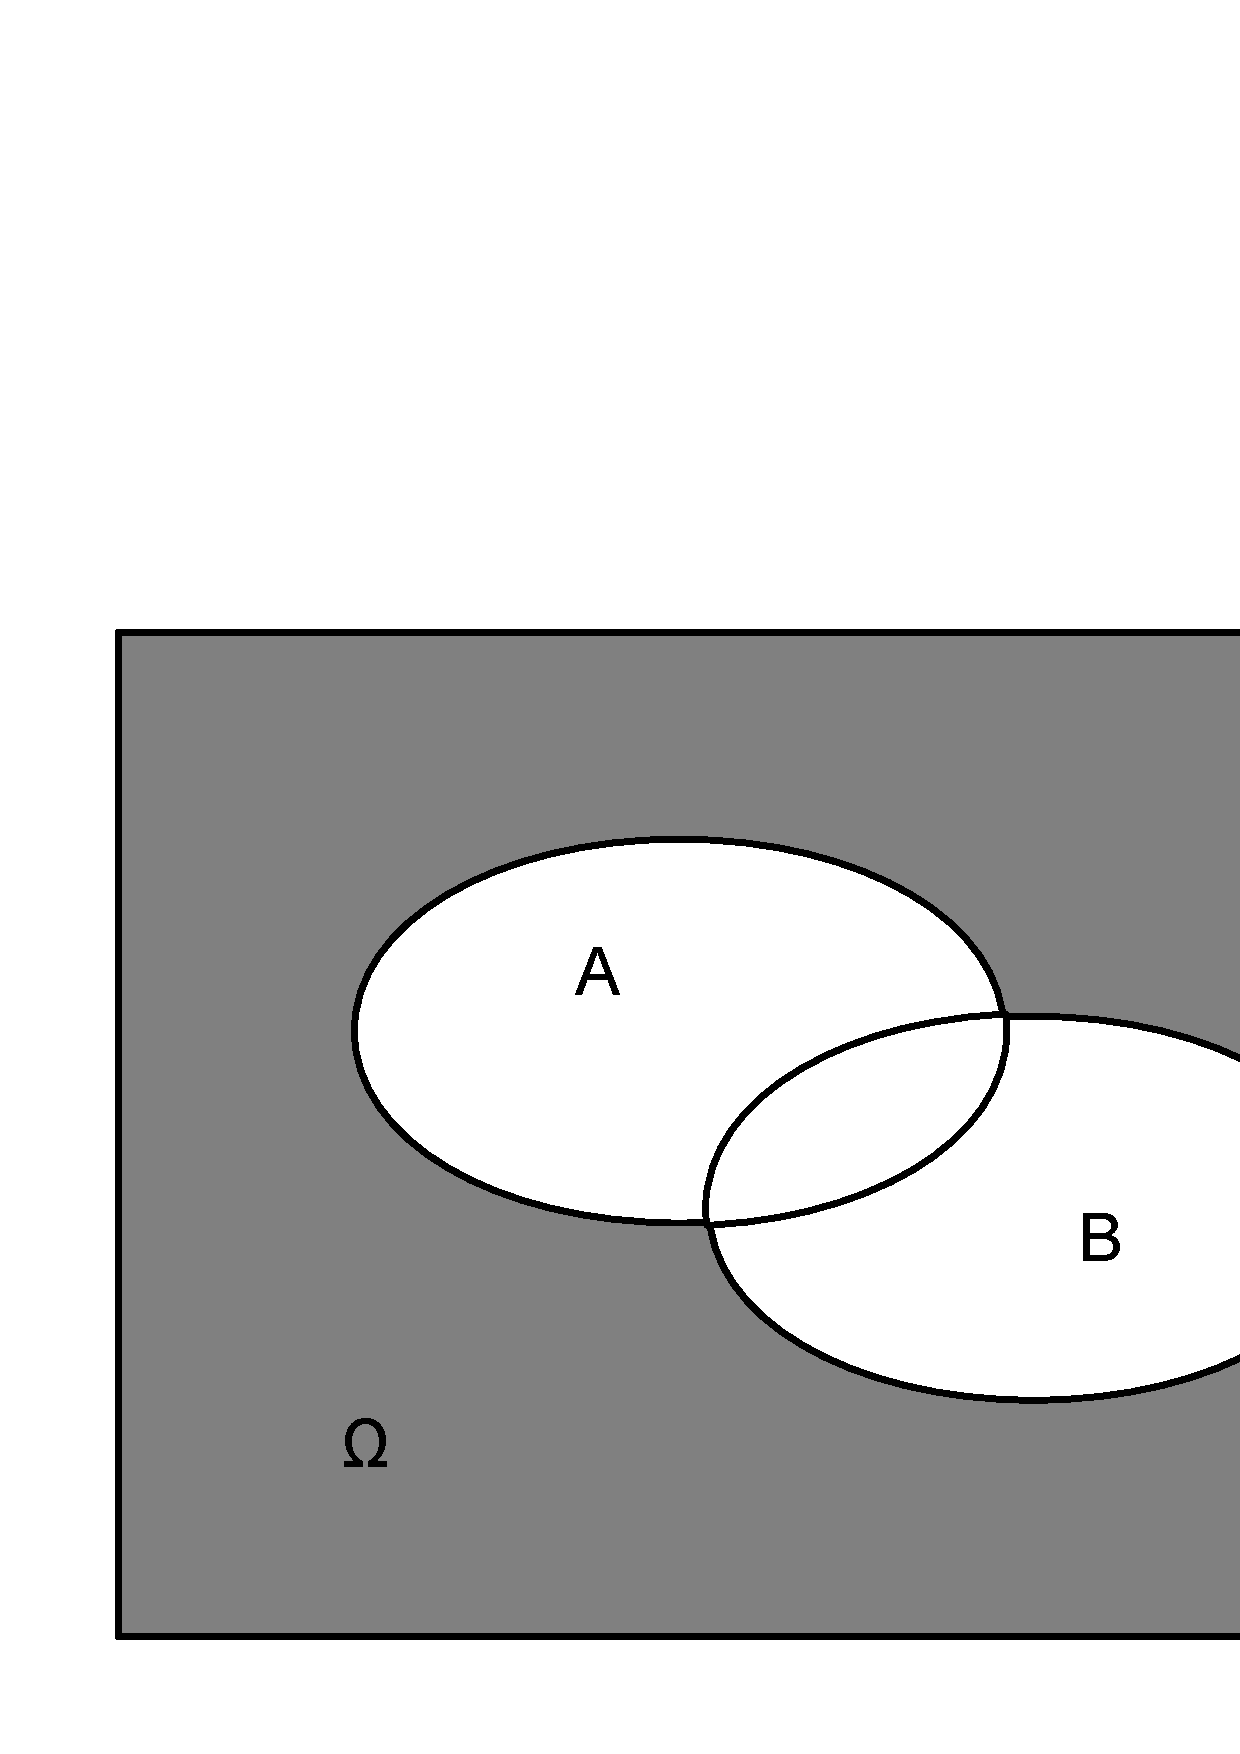
\includegraphics[width=3.0in]{figures/A_union_B_comp}}
\quad
\subfigure[$\left( A \cap B \right)^c = A^c \cup B^c$]{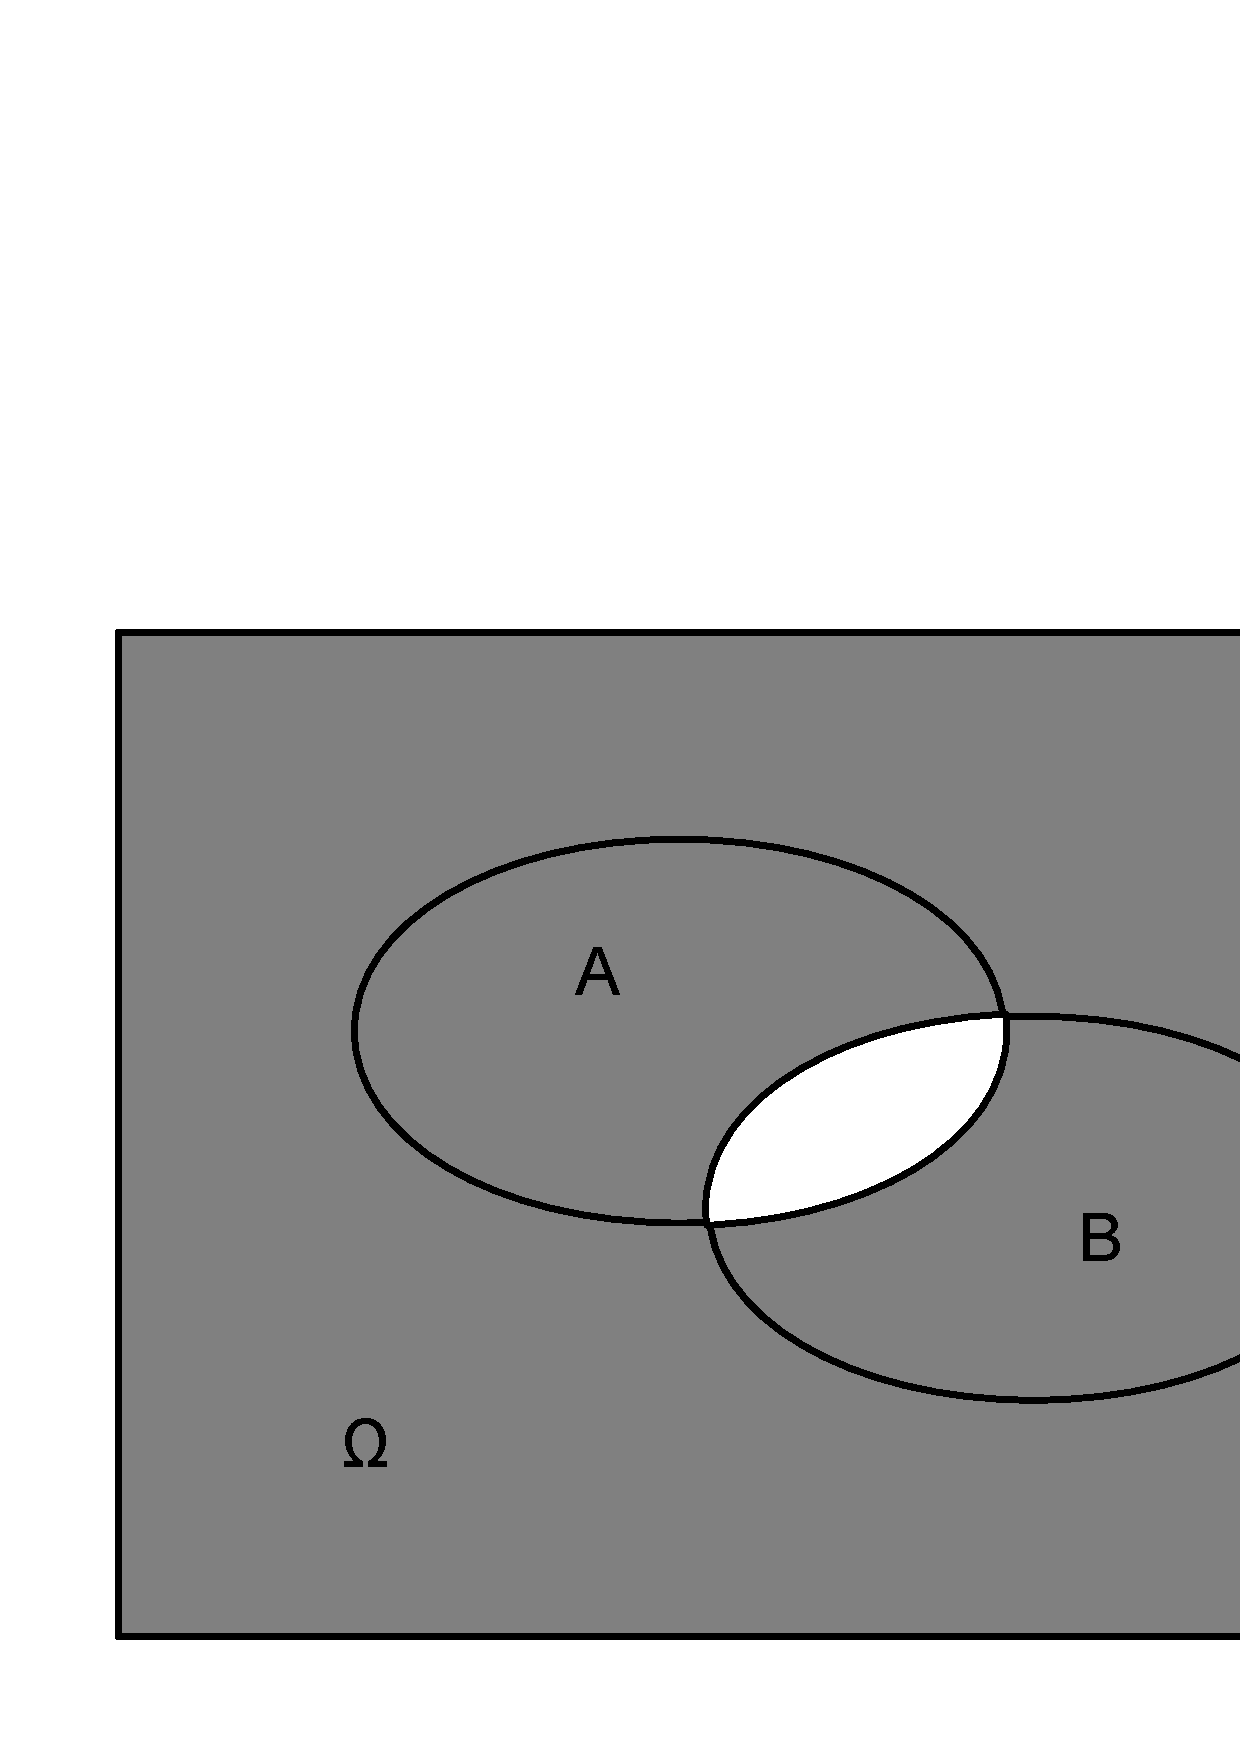
\includegraphics[width=3.0in]{figures/A_inter_B_comp} }
}
\caption{These  Venn diagram illustrate De~Morgan's Laws.} \label{F:DeMorganslaws}
\end{figure}


%\begin{figure}[htpb]
%\caption{Universal set $\Omega$, a set $A$ such that $A \subset \Omega$ (read: $A$ is a subset of $\Omega$ or $A$ is contained in $\Omega$), another set $B$ with $B \subset \Omega$,  the set $A \setminus B$ (read: $A$ (set)minus $B$ or $A$ that is not in $B$), the set $A \cap B$ (read: $A$ intersection $B$), the set $A \cup B$ (read: $A$ union $B$) and the set $A^c$ (read: complement of $A$) which is defined as $\Omega \setminus A$.}
%\vspace{6cm}
%\end{figure}

\begin{classwork}[Fruits and colours]
Consider a set of fruits $F=\{\text{orange}, \text{banana}, \text{apple}\}$ and a set of colours $C = \{\text{red}, \text{green}, \text{blue}, \text{orange}\}$.  Then,
\begin{enumerate}
\item $F \cap C = $
\item $F \cup C = $
\item $F \setminus C = $
\item $C \setminus F = $
\end{enumerate}
\end{classwork}




\begin{classwork}[Subsets of a universal set]
Suppose we are given a universal set $U$, and three of its subsets, $A$, $B$ and $C$.  Also suppose that $A \subset B \subset C$.  Find the circumstances, if any, under which each of the following statements is true (T) and justify your answer:

\begin{tabular*}{5.5in}{@{\extracolsep{\fill}}l l l l}
(1) $C \subset B$ & T when $B=C$
&(2) $A \subset C$ & T by assumption\\
(3) $C \subset \emptyset$ & T when $A=B=C=\emptyset$
&(4) $\emptyset \subset A$& T always \\
(5) $C \subset U$ & T by assumption
&(6) $U \subset A$ & T when $A=B=C=U$\\
\end{tabular*}
\end{classwork}

\section{Exercises}\label{xSets}

\begin{ExerciseList}

\Exercise
Let $\Omega$ be the universal set of students, lecturers and tutors involved in a course.

Now consider the following subsets:
\begin{itemize}
\item The set of 50 students, $S\,=\, \{S_1,\, S_2,\, S_2,\,\dots \, S_{50}\}$.

\item The set of 3 lecturers, $L\,=\, \{L_1,\,L_2,\, L_3\}$.

\item The set of 4 tutors, $T\,=\, \{T_1,\,T_2,\, T_3,\, L_3\}$.
\end{itemize}
Note that one of the lecturers also tutors in the course. Find the following sets:

\bcols{2}\be

\item[(a)] $T \cap L$

\item[(b)] $T \cap S$

\item[(c)] $T \cup L$

\item[(d)] $T \cup L \cup S$

\item[(e)] $S^c$

\item[(f)] $S \cap L$

\item[(g)] $S^c\cap L$

\item[(h)] $T^c$

\item[(i)] $T^c\cap L$


\item[(j)] $T^c\cap T$

\ee\ecols

\Answer
By operating with $\Omega$, $T$, $L$ and $S$ we can obtain the answers as follows:

{\bcols{2}\be

\item[(a)] $T \cap L\,=\, \{L_3\}$

\item[(b)] $T \cap S\,=\, \emptyset$

\item[(c)] $T \cup L\,=\, \{ T_1,\,T_2,\, T_3,\, L_3,\, L_1,\, L_2\}$

\item[(d)] $T \cup L \cup S\,=\, \Omega$

\item[(e)] $S^c \,=\,\{ T_1,\,T_2,\, T_3,\, L_3,\, L_1,\, L_2\} $

\item[(f)] $S \cap L\,=\, \emptyset$

\item[(g)] $S^c\cap L\,=\,\{L_1,\, L_2,\,L_3\}\,=\, L $

\item[(h)] $T^c\,=\,\{L_1,\, L_2,\,S_1,\, S_2,\, S_2,\,\dots \, S_{50}\}  $

\item[(i)] $T^c \cap L\,=\,\{L_1,\, L_2\} $


\item[(j)] $T^c\cap T\,=\, \emptyset$

\ee\ecols
}

%\begin{Exercise}[title={Venn Diagrams 1}]
\Exercise
Using Venn diagram, sketch and check the rule:

$A\cup(B\cap C)\,=\,(A\cup B)\cap (A\cup C)$

\Exercise
Using Venn diagram, sketch and check the rule:

$A\cap(B\cup C)\,=\,(A\cap B)\cup(A\cap C)$

%\end{Exercise}
\Answer
We can check $A\cup(B\cap C)\,=\,(A\cup B)\cap (A\cup C)$ from the following sketch:

\begin{center}
%\subfloat[$A\cup(B\cap C)$]
{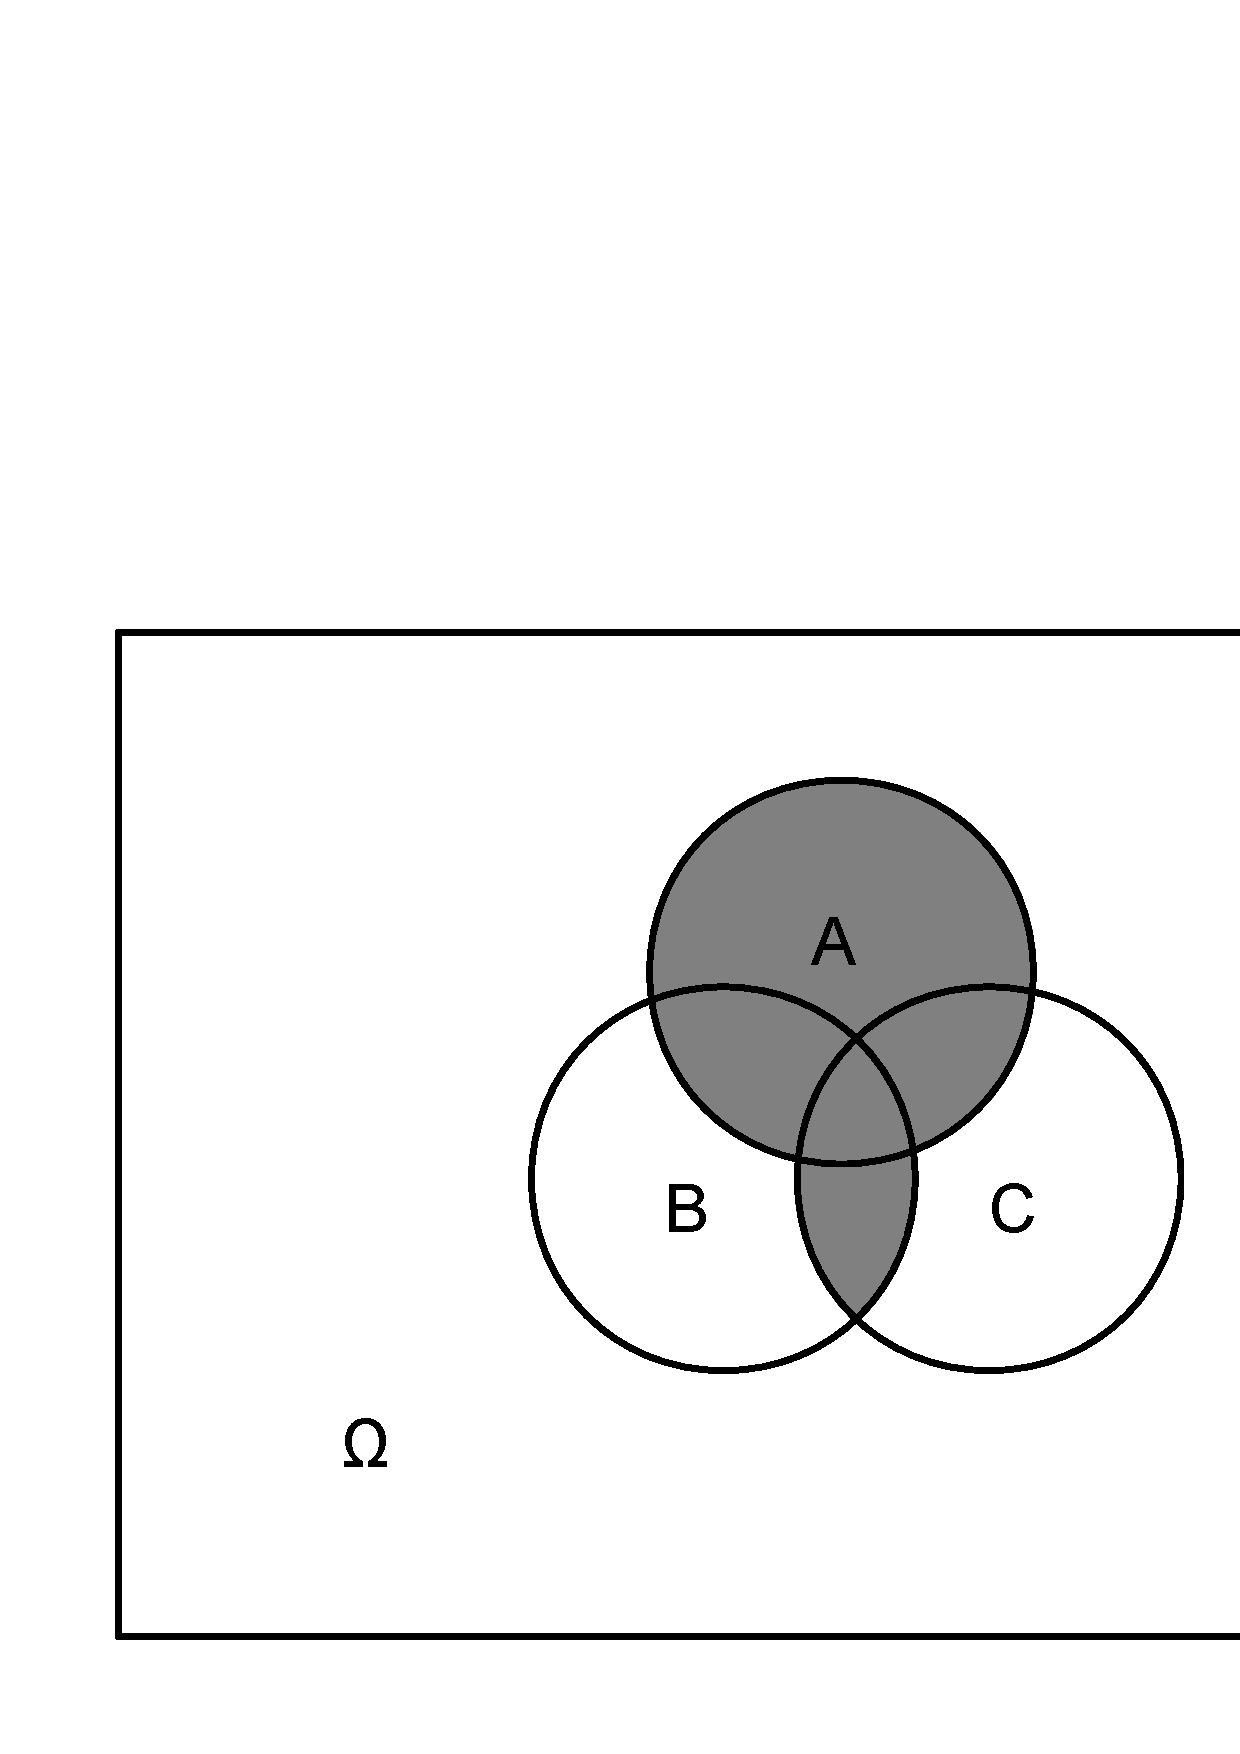
\includegraphics[width=5cm]{figures/ABC1}}
\end{center}

\Answer
We can check $A\cap(B\cup C)\,=\,(A\cap B)\cup(A\cap C)$ from the following sketch:

%\subfloat[$A\cap(B\cup C)$]
We can check $A\cup(B\cap C)\,=\,(A\cup B)\cap (A\cup C)$ from the following sketch:
\begin{center}
{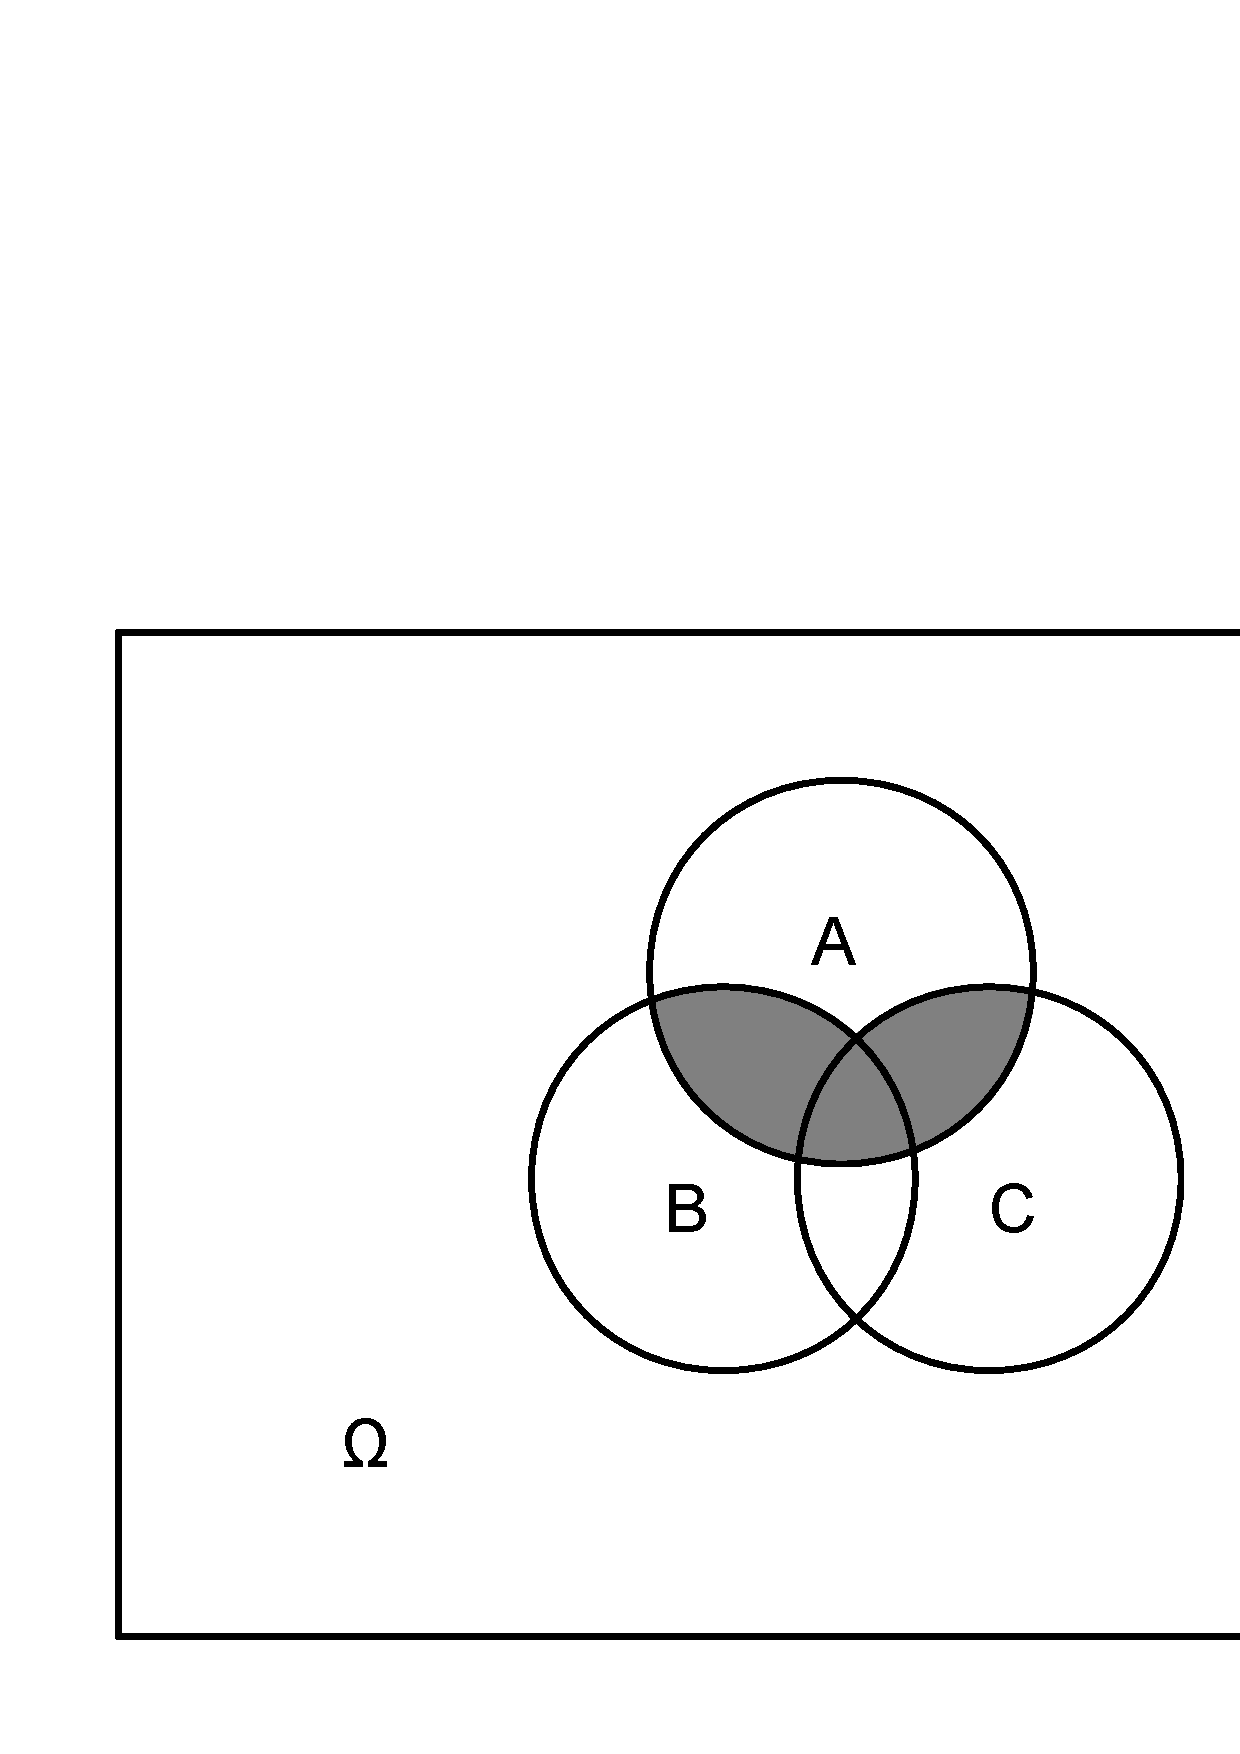
\includegraphics[width=5cm]{figures/ABC2}}
\end{center}

%question 2

%\begin{Exercise}[title={Venn Diagrams 2}]
\Exercise
Using a Venn diagram, illustrate the idea that  $A\subseteq B$ if and only if $A\cup B=B$.
%\end{Exercise}
\Answer
To illustrate the idea that $A\subseteq B$ if and only if $A\cup B=B$, we need to illustrate two implications:
\begin{enumerate}
\item if $A\subseteq B$ then  $A\cup B=B$ and
\item if  $A\cup B=B$ then $A\subseteq B$.
\end{enumerate}
The folowing Venn diagram illustrates the two implications clearly.
\begin{center}
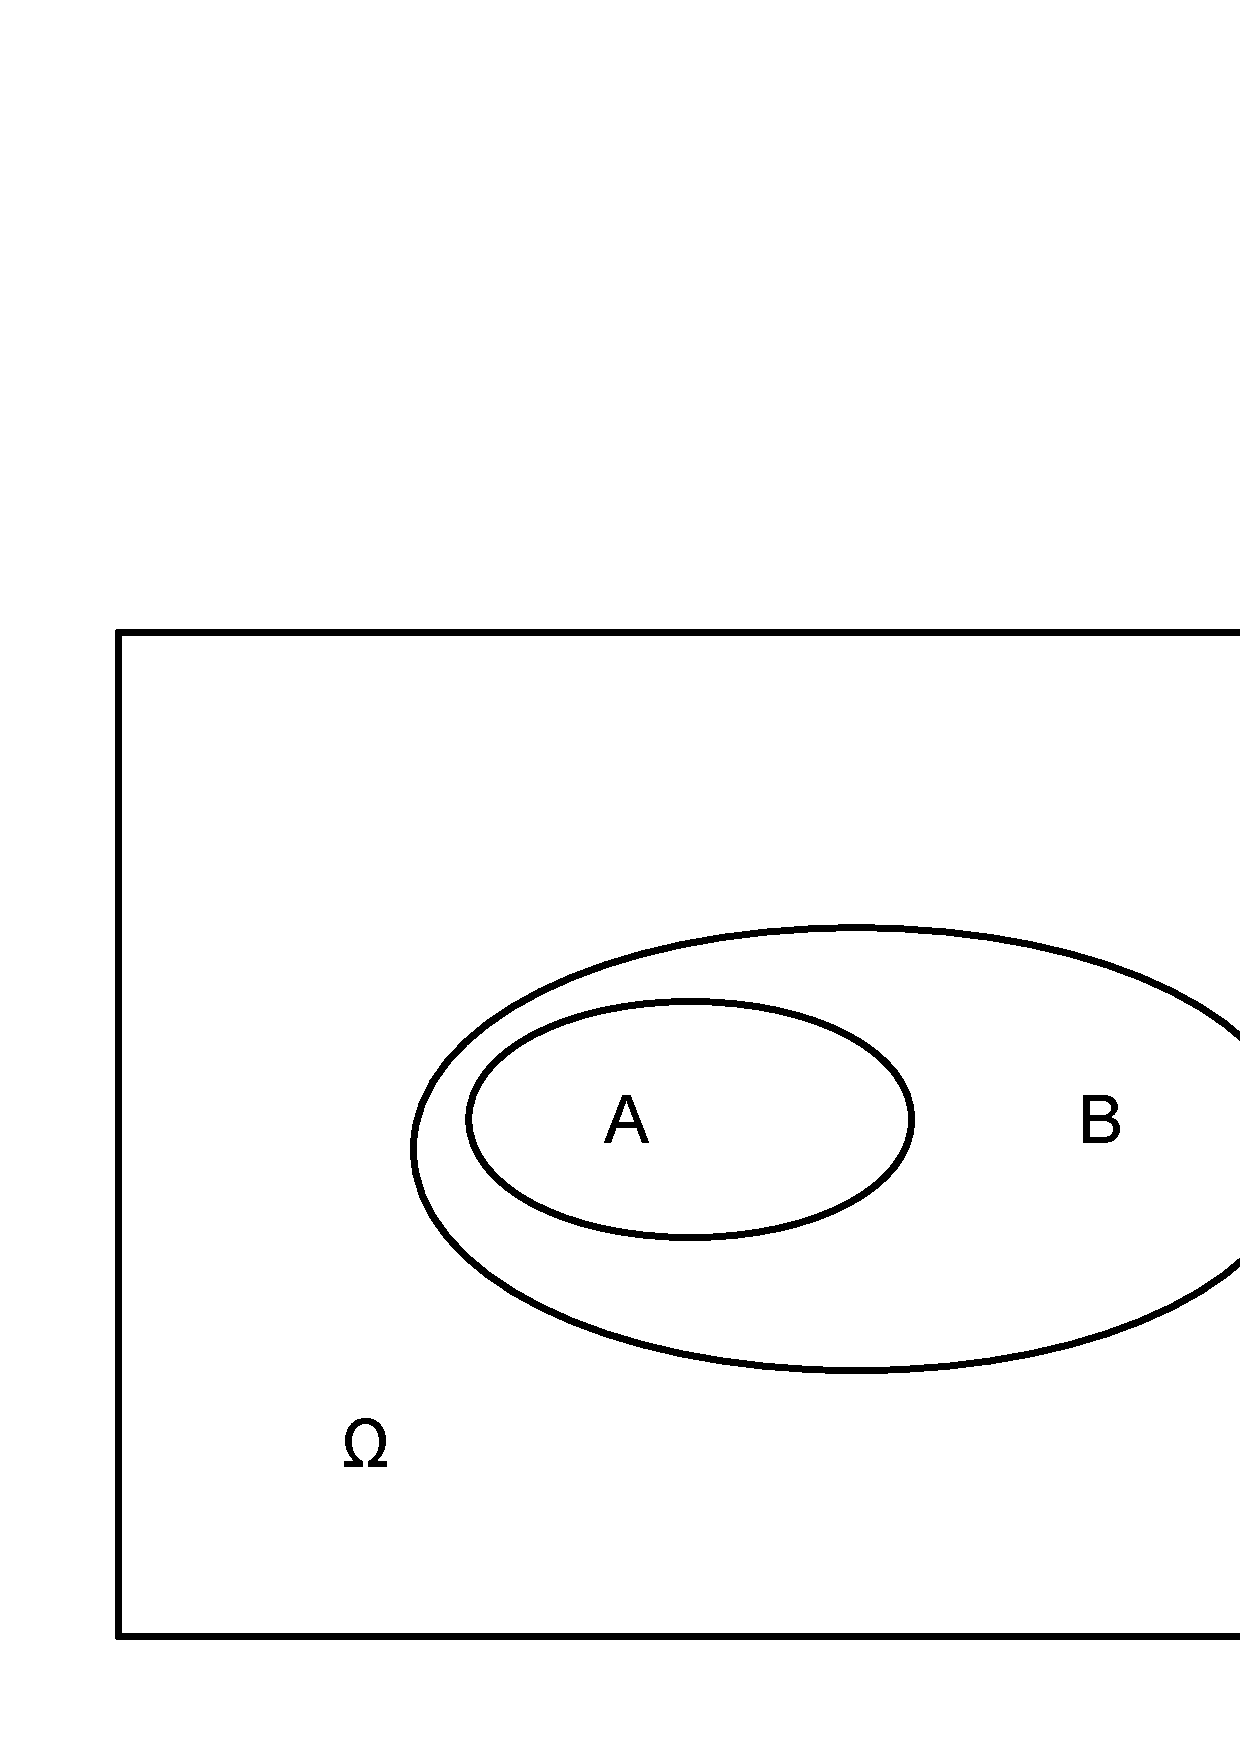
\includegraphics[width=6cm]{figures/AB}
\end{center}

\end{ExerciseList}

\begin{framed}
\begin{tabular}{rcl}
SET SUMMARY\\ \\
$\{a_1,a_2,\dots,a_n\}$& $-$& a set containing the elements, $a_1,a_2,\dots,a_n$.\\
$a\in A$ &$-$& $a$ is an element of the set $A$.\\
$A\subseteq B$ &$-$& the set $A$ is a subset of $B$.\\
$A\cup B$ &$-$& ``union'', meaning the set of all elements which are in $A$ or $B$, \\
& & \ \ or both.\\
$A\cap B$ &$-$& ``intersection'', meaning the set of all elements in both $A$ and $B$.\\
$\{\}$ or $\emptyset$ &$-$& empty set.\\
$\Omega $ &$-$& universal set.  \\
$A^c $ &$-$& the complement of $A$, meaning the set of all elements in $\Omega$,\\
& & \ \ the universal set, which are not in $A$.\\
\end{tabular}
\end{framed}

%\remove{
\section{Natural Numbers, Integers and Rational Numbers}\label{S:NatIntRatNumbers}

We denote the number of elements in a set named $B$ by:
\[
\boxed{
\# B := \text{Number of elements in the set $B$}
} \ .
\]
In fact, the Hindu-Arab numerals we have inherited are based on this intuition of the size of a collection.  The elements of the set of {\bf natural numbers}:
\[
\boxed{
\Nz := \{1,2,3,4,\ldots \}
} \ , \text{may be defined using $\#$ as follows:}
\]
\begin{flalign*}
1 &:= \#\{\star \} = \# \{\bullet\}= \#\{\alpha\}=\#\{\{\bullet\}\} = \#\{\{\bullet,\bullet'\}\}= \ldots,\\
2 &:= \#\{\star',\star \} = \# \{\bullet, \circ\}= \#\{\alpha,\omega\} = \#\{\{\circ\},\{\alpha,\star,\bullet\}\}=\ldots,\\
\vdots &
\end{flalign*}
For our example sets, $A=\{\circ,\bullet\}$ and the set of Greek alphabets $\BB{\E{G}}$, $\# A = 2$ and $\# \BB{\E{G}} = 22$.  The number zero may be defined as the size of an empty set:
\[
0 := \# \emptyset = \#\{\}
\]
The set of {\bf non-negative integers} is:
\[
\boxed{
\Zz_+ := \Nz \cup \{0\} = \{0,1,2,3,\ldots\}
} \ .
\]

A {\bf product set} is the {\bf Cartesian product} ($\times$) of two or more possibly distinct sets:
\[
\boxed{
A \times B := \{(a,b): a \in A \text{ and } b \in B \}
}
\]
For example, if $A=\{\circ,\bullet\}$ and $B=\{\star\}$, then $A\times B = \{(\circ,\star), (\bullet,\star)\}$.  Elements of $A \times B$ are called {\bf ordered pairs}.

The binary arithmetic operation of {\bf addition} ($+$) between a pair of non-negative integers $c,d \in \Zz_+$ can be defined via sizes of disjoint sets.  Suppose, $c=\#C$, $d=\#D$ and $C \cap D = \emptyset$, then:
\[
c+d = \#C + \#D := \# (C \cup D) \ .
\]
For example,  if $A=\{\circ,\bullet\}$ and $B=\{\star\}$, then $A \cap B=\emptyset$ and $\#A + \#B = \#(A \cup B) \iff 2+1=3$.

The binary arithmetic operation of {\bf multiplication} ($\cdot$) between a pair of non-negative integers $c,d \in \Zz_+$ can be defined via sizes of product sets.  Suppose, $c=\#C$, $d=\#D$, then:
\[
c \cdot d = \#C \cdot \#D := \# (C \times D) \ .
\]
For example,  if $A=\{\circ,\bullet\}$ and $B=\{\star\}$, then $\#A \cdot \#B = \#(A \times B) \iff 2 \cdot 1=2$.

More generally, a product set of $A_1,A_2,\ldots,A_m$ is:
\[
\boxed{
A_1 \times A_2 \times \cdots \times A_m := \{(a_1,a_2,\ldots,a_{m}): a_1 \in A_1, a_2 \in A_2, \ldots, a_{m} \in A_m \}
}
\]
Elements of an $m$-product set are called {\bf ordered $m$-tuples}.  When we take the product of the same set we abbreviate as follows:
\[
\boxed{
A^m := \underset{m \text{ times}}{\underbrace{A \times A \times \cdots \times A}} := \{(a_1,a_2,\ldots,a_m): a_1 \in A, a_2 \in A, \ldots, a_{m} \in A \}
}
\]
\begin{classwork}[Cartesian product of sets]
1.~Let $A=\{\circ, \bullet \}$.  What are the elements of $A^2$?  2.~Suppose $\# A = 2$ and $\# B = 3$.  What is $\# (A \times B)$?  3.~Suppose $\# A_1 = s_1, \# A_2 = s_2, \ldots, \# A_m = s_m$.  What is $\# (A_1 \times A_2 \times \cdots \times A_m)$?
\vspace{4cm}
\end{classwork}

Now, let's recall the definition of a function.  A {\bf function} is a ``mapping" that associates each element in some set $\Xz$ (the domain) to exactly one element in some set $\Yz$ (the range). Two different elements in $\Xz$ can be mapped to or associated with the same element in $\Yz$, and not every element in $\Yz$ needs to be mapped.  Suppose $x \in \Xz$. Then we say ${f(x)=y \in \Yz}$ is the {\bf image} of $x$.  To emphasise that $f$ is a {\bf function} from $\Xz \ni x$ to $\Yz \ni y$, we write:
$$\boxed{f(x)=y:\Xz \to \Yz} \ .$$
And for some $y \in \Yz$, we call the set:
$$\boxed{f^{[-1]}(y) := \{x \in \Xz : f(x)=y \} \subset \Xz} \ ,$$
the {\bf pre-image} or {\bf inverse image} of $y$, and
$$\boxed{f^{[-1]} := f^{[-1]}(y \in \Yz) = X \subset \Xz} \ ,$$
as the {\bf inverse} of $f$.

\begin{figure}[htpb]
\caption{A function $f$ (``father of'') from $\Xz$ (a set of children) to $\Yz$ (their fathers) and its inverse (``children of'').\label{F:function}}
\vspace{4cm}
\end{figure}

We motivated the non-negative integers $\Zz_+$ via the size of a set.  With the notion of two directions ($+$ and $-$) and the magnitude of the current position from the origin zero ($0$) of a dynamic entity, we can motivate the set of {\bf integers}:
$$\boxed{\Zz := \{\ldots,-3,-2,-1,0,+1,+2,+3,\ldots\}} \ .$$
The integers with a {\bf minus} or {\bf negative sign} ($-$) before them are called negative integers and those with a {\bf plus} or {\bf positive sign} ($+$) before them are called positive integers.  Conventionally, $+$ signs are dropped.  Some examples of functions you may have encountered are {\bf arithmetic operations} such as {\bf addition} ($+$), {\bf subtraction} ($-$), {\bf multiplication} ($\cdot$) and {\bf division} ($/$) of ordered pairs of integers.  The reader is assumed to be familiar with such arithmetic operations with pairs of integers.  Every integer is either positive, negative, or zero.  In terms of this we define the notion of {\bf order}.  We say an integer $a$ is {\bf less than} an integer $b$ and write $a < b$ if $b-a$ is positive.  We say an integer $a$ is {\bf less than or equal to} an integer $b$ and write $a \leq b$ if $b-a$ is positive or zero.  Finally, we say that $a$ is greater than $b$ and write $a > b$ if $b<a$.  Similarly, $a$ is greater than equal to $b$, i.e.~$a \geq b$, if $b \leq a$.  The set of integers are {\bf well-ordered}, i.e., for every integer $a$ there is a next largest integer $a+1$.

\begin{classwork}[Addition over integers]\label{CW:AdditionMapAndItsInverseMap}
Consider the set of integers $\Zz = \{\ldots,-3,-2,-1,0,1,2,3,\ldots\}$.  Try to set up the arithmetic operation of addition as a function.  The domain for addition is the Cartesian product of $\Zz$:
\[
 \Zz^2 := \Zz \times \Zz := \{(a,b) : a \in \Zz, b \in \Zz \}
\]
What is its range ?
\[
+ : \Zz \times \Zz \to
\]
\begin{figure}[htpb]
\caption{A pictorial depiction of addition and its inverse.  The domain is plotted in orthogonal  {\bf Cartesian coordinates}.\label{F:Addfunction}}
\vspace{5cm}
\end{figure}
\end{classwork}

If the magnitude of the entity's position is measured in units (e.g.~meters) that can be rationally divided into $q$ pieces with $q \in \Nz$, then we have the set of rational numbers:
\[
\Qz := \{ {p}/{q} : p \in \Zz, q \in \Zz \setminus \{0\} \}
\]
The expressions $p/q$ and $p'/q'$ denote the same rational number if and only if $p \cdot q'=p' \cdot q$.  Every rational number has a unique irreducible expression $p/q$, where $q$ is positive and as small as possible.  For example, $1/2$, $2/4$, $3/6$, and $1001/2002$ are different expressions for the same rational number whose irreducible unique expression is $1/2$.

Addition and multiplication are defined for rational numbers by:
\[
\frac{p}{q} + \frac{p'}{q'} = \frac{p \cdot q' + p' \cdot q}{q \cdot q'}
\qquad \text{and} \qquad \frac{p}{q} \cdot \frac{p'}{q'} = \frac{p \cdot p'}{q \cdot q'} \ .
\]
The rational numbers form a {\bf field} under the operations of addition and multiplication defined above in terms of addition and multiplication over integers.  This means that the following properties are satisfied:
\begin{enumerate}
\item Addition and multiplication are each {\bf commutative}
\[ a+b = b+a, \qquad a \cdot b = b \cdot a \ , \]
and associative
\[
a + (b + c) = (a + b) + c, \qquad a \cdot (b \cdot c) = (a \cdot b) \cdot c \ .
\]
\item Multiplication {\bf distributes} over addition
\[
a \cdot (b+c) = (a \cdot b) + (a \cdot c) \ .
\]
\item $0$ is the {\bf additive identity} and $1$ is the multiplicative identity
\[
0+a=a \qquad \text{and} \qquad 1 \cdot a = a \ .
\]
\item Every rational number $a$ has a negative, $a+(-a)=0$ and every non-zero rational number $a$ has a reciprocal, $a \cdot 1/a = 1$.
\end{enumerate}
The field axioms imply the usual laws of arithmetic and allow subtraction and division to be defined in terms of addition and multiplication as follows:
\[
\frac{p}{q} - \frac{p'}{q'} := \frac{p}{q} + \frac{-p'}{q'}
\qquad \text{and} \qquad  \frac{p}{q} / \frac{p'}{q'} := \frac{p}{q} \cdot \frac{q'}{p'}, \quad \text{provided $p' \neq 0$} \ .
\]
We will see later that the theory of finite fields is necessary for the study of pseudo-random number generators (PRNGs) and PRNGs are the heart-beat of randomness and statistics with computers.

%\afterpage{clearpage}

%You should at least have a  ``working knowledge'' of the following topics as they constitute the foundational kernels of statistical reasoning:
%\begin{itemize}
%\item Finite and infinite sequences of rational numbers
%\item Limits, Cauchy sequences of rational numbers and the real number system
%\item Continuous functions, derivatives and differentiable functions
%\end{itemize}
\section{Real Numbers}\label{S:Reals}
Unlike rational numbers which are expressible in their reduced forms by $p/q$, it is fairly tricky to define or express real numbers.  It is possible to define real numbers formally and constructively via equivalence classes of Cauchy sequence of rational numbers.  For this all we need are notions of (1) infinity, (2) sequence of rational numbers and (3) distance between any two rational numbers in an infinite sequence of them.  These are topics usually covered in an introductory course in real analysis and are necessary for a firm  foundation in computational statistics.  Instead of a formal constructive definition of real numbers, we give a more concrete one via decimal expansions.  See Donald E.~Knuth's treatment [{\em Art of Computer Programming, Vol.~I, Fundamental Algorithms}, 3rd Ed., 1997, pp.~21-25] for a fuller story.  A {\bf real number} is a numerical quantity $x$ that has a decimal expansion:
\[
x = n+ 0.d_1d_2d_3 \ldots \ , \text{ where, each } d_i \in \{0,1,\ldots,9\}, n \in \Zz \ ,
\]
and the sequence $ 0.d_1d_2d_3 \ldots$ does not terminate with infinitely many consecutive $9$s.  By the above decimal representation, the following arbitrarily accurate enclosure of the real number $x$ by rational numbers is implied:
\[
n+\frac{d_1}{10}+\frac{d_2}{100}+\cdots+\frac{d_k}{10^k} =: \underline{x}_k \leq x < \overline{x}_k :=
n+\frac{d_1}{10}+\frac{d_2}{100}+\cdots+\frac{d_k}{10^k}+\frac{1}{10^k}
\]
for every $k \in \Nz$.  Thus, rational arithmetic ($+,-,\cdot,/$) can be extended with arbitrary precision to any ordered pair of real numbers $x$ and $y$ by operations on their rational enclosures $\underline{x}, \overline{x}$ and $\underline{y}, \overline{y}$.

Some examples of real numbers that are not rational ({\bf irrational numbers}) are:
\begin{flalign*}
\sqrt{2}=1.41421356237309\ldots & \text{the side length of a square with area of $2$ units}\\
\pi=3.14159265358979\ldots  & \text{the ratio of the circumference to diameter of a circle} \\
e=2.71828182845904\ldots & \text{Euler's constant}
\end{flalign*}
We can think of $\pi$ as being enclosed by the following pairs of rational numbers:
\begin{flalign*}
3 +\frac{1}{10} =: \underline{\pi}_{1} \leq &\pi < \overline{\pi}_{1} := 3 + \frac{1}{10} + \frac{1}{10^{1}} \\
3 +\frac{1}{10} + \frac{4}{100} =: \underline{\pi}_{2} \leq &\pi < \overline{\pi}_{2} := 3 + \frac{1}{10} + \frac{4}{100}+\frac{1}{100} \\
3 +\frac{1}{10} + \frac{4}{100} + \frac{1}{10^3} =: \underline{\pi}_{3} \leq &\pi < \overline{\pi}_{3} := 3 + \frac{1}{10} + \frac{4}{100}+ \frac{1}{10^3}+\frac{1}{10^3} \\
&\vdots \\
3.14159265358979 =: \underline{\pi}_{14} \leq &\pi < \overline{\pi}_{14} := 3.14159265358979 + \frac{1}{10^{14}} \\
& \vdots
\end{flalign*}

Think of the real number system as the continuum of points that make up a line, as shown in ~\hyperref[F:linesegment]{Figure~\ref*{F:linesegment}}.
\begin{figure}[htpb]
\caption{A depiction of the real line segment $[-10,10]$.\label{F:linesegment}}
\vspace{3cm}
\end{figure}

Let $y$ and $z$ be two real numbers such that $y \leq z$.  Then, the {\bf closed interval} $[y,z]$ is the set of real numbers $x$ such that $y \leq x \leq z$:
\[
[y,z] := \{ x: y \leq x \leq z \} \ .
\]
The {\bf half-open interval} $(y,z]$ or $[y,z)$ and the {\bf open interval} $(y,z)$  are defined analogously:
\begin{flalign*}
(y,z] &:= \{ x: y < x \leq z \} \ , \\
[y,z) &:= \{ x: y \leq x < z \} \ , \\
(y,z) &:=  \{ x: y < x < z \} \ .
\end{flalign*}
We also allow $y$ to be {\bf minus infinity} (denoted $-\infty$) or $z$ to be {\bf infinity} (denoted $\infty$) at an open endpoint of an interval, meaning that there is no lower or upper bound.  With this allowance we get the set of {\bf real numbers} $\Rz := (-\infty,\infty)$, the {\bf non-negative real numbers} $\Rz_+:=[0,\infty)$ and the {\bf positive real numbers} $\Rz_{>0}(0,\infty)$ as follows:
\begin{flalign*}
\Rz &:= (-\infty,\infty) =  \{ x: -\infty < x < \infty \} \ , \\
\Rz_+ &:= [0,\infty) =  \{ x: 0 \leq x < \infty \} \ , \\
\Rz_{>0} &:= [0,\infty) =  \{ x: 0 < x < \infty \} \ . \\
\end{flalign*}
For a positive real number $b \in \Rz_{>0}$ and an integer $n \in \Zz$, the $n$-th {\bf power} or {\bf exponent} of $b$ is:
\[
b^0=1, \qquad b^n = b^{n-1} \cdot b \quad \text{if $n>0$}, \qquad b^n=b^{n+1}/b  \quad \text{if $n<0$} \ .
\]
The following {\bf laws of exponents} hold by mathematical induction when $m,n \in \Zz$:
\[
b^{m+n} = b^m \cdot b^n, \qquad \left( b^m \right)^n = b^{m \cdot n} \ .
\]
If $y \in \Rz$ and $m \in \Nz$, the unique positive real number $z \in \Rz_{>0}$ such that $z^m=y$ is called the {\bf $m$-th root of $y$} and denoted by $\sqrt[m]{y}$, i.e.,
\[
z^m=y \implies z=\sqrt[m]{y} \ .
\]
For a rational number $r=p/q \in \Qz$, we define the $r$-th power of $b \in \Rz$ as follows:
\[
b^r = b^{p/q} := \sqrt[q]{b^p}
\]
The laws of exponents hold for this definition and different expressions for the same rational number $r=ap/aq$ yield the same power, i.e.,~$ b^{p/q}= b^{ap/aq}$.  Recall that a real number $x=n+ 0.d_1d_2d_3\ldots \in \Rz$ can be arbitrarily precisely enclosed by the rational numbers $\underline{x}_k:=n+\frac{d_1}{10}+\frac{d_2}{100}+\cdots+\frac{d_k}{10^k}$ and $\overline{x}_k:=n+\frac{d_1}{10}+\frac{d_2}{100}+\cdots+\frac{d_k}{10^k}+\frac{1}{10^k}$ by increasing $k$.  Suppose first that $b>1$.  Then, using rational powers, we can enclose $b^x$,
\[
b^{n+\frac{d_1}{10}+\frac{d_2}{100}+\cdots+\frac{d_k}{10^k}} =: b^{\underline{x}_k} \leq b^{x} < b^{\overline{x}_k} := b^{n+\frac{d_1}{10}+\frac{d_2}{100}+\cdots+\frac{d_k}{10^k}+\frac{1}{10^k}} \ ,
\]
within an interval of width $b^{n+\frac{d_1}{10}+\frac{d_2}{100}+\cdots+\frac{d_k}{10^k}} \left(b^{\frac{1}{10^k}}-1 \right) < b^{n+1}(b-1)/10^k$.  By taking a large enough $k$ we can evaluate $b^x$ to any accuracy.  Finally, when $b<1$ we define $b^x : = (1/b)^x$ and when $b=0$, $b^x := 1$.

Suppose $y \in \Rz_{>0}$ and $b \in \Rz \setminus \{1\}$ then the real number $x$ such that $y=b^x$ is called the {\bf logarithm of $y$ to the base $b$} and we write this as:
\[
y=b^x \iff x = \log_b{y}
\]
The definition implies:
\[
x = \log_b (b^x) = b^{\log_b x} \ ,
\]
and the laws of exponents imply:
\begin{flalign*}
\log_b(xy) &= \log_b{x} + \log_b{y}, \quad \text{if} \quad x >0, \ y >0 \ \text{ and} \\
\log_b \left( c^y \right) &= y \log_b c, \quad \text{if} \quad c > 0 \ .
\end{flalign*}
The {\bf common logarithm} is $\log_{10}(y)$, the {\bf binary logarithm} is $\log_2(y)$ and the {\bf natural logarithm} is $\log_e(y)$, where $e$ is the Euler's constant.  Since we will mostly work with $\log_e(y)$ we use $\log(y)$ to mean $\log_e(y)$.  You are assumed to be familiar with trigonometric functions ($\sin(x)$, $\cos(x)$, $\tan(x)$, $\ldots$).  We sometimes denote the special power function $e^y$ by $\exp(y)$.

Familiar extremal elements of a set of real numbers, say $A$, are the following:
\[
\boxed{
\max{A} := \text{greatest element in $A$}
}
\]
For example, $\max \{1,4,-9,345\} = 345$, $\max [-93.8889,1002.786] = 1002.786$.
\[
\boxed{
\min{A} := \text{least element in $A$}
}
\]
For example, $\min \{1,4,-9,345\} = -9$, $\min [-93.8889,1002.786] = -93.8889$.  We need a slightly more sophisticated notion for the extremal elements of a set $A$ that may not belong to $A$.  We say that a real number $x$ is a {\bf lower bound} for a non-empty set of real numbers $A$, provided $x \leq a$ for every $a \in A$.  We say that the set $A$ is {\bf bounded below} if it has at least one lower bound.  A lower bound is the {\bf greatest lower bound} if it is at least as large as any other lower bound.  The greatest lower bound of a set of real numbers $A$ is called the {\bf infimum} of $A$ and is denoted by:
\[
\boxed{
\inf{A} := \text{greatest lower bound of $A$}
}
\]
For example, $\inf (0,1) = 0$ and $\inf \{ 10.333 \cup [-99,1001.33) \} = -99$.  We similarly define the {\bf least upper bound} of a non-empty set of real numbers $A$ to be the {\bf supremum} of $A$ and denote it as:
\[
\boxed{
\sup{A} := \text{least upper bound of $A$}
}
\]
For example, $\sup (0,1) = 1$ and $\sup \{ 10.333 \cup [-99,1001.33) \} = 1001.33$.  By convention, we define $\inf \emptyset := \infty$, $\sup \emptyset := - \infty$.  Finally, if a set $A$ is not bounded below then $\inf A := - \infty$ and if a set $A$ is not bounded above then $\sup A := \infty$.
\begin{table}[htb]
\centering
{\small
\begin{tabular}{| l | l |}
\hline
Symbol & Meaning\\ \hline
$A = \{ \star, \circ, \bullet \}$& $A$ is a set containing the elements $\star$, $\circ$ and $\bullet$ \\
$\circ \in A$ & $\circ$ belongs to $A$ or $\circ$ is an element of $A$\\
$A \ni \circ$ & $\circ$ belongs to $A$ or $\circ$ is an element of $A$\\
$\odot \notin A$& $\odot$ does not belong to $A$ \\
$\# A$& Size of the set $A$, for e.g.~$\#\{ \star, \circ, \bullet, \odot \}=4$\\
$\Nz$& The set of natural numbers $\{1,2,3,\ldots\}$\\
$\Zz$&The set of integers $\{\ldots,-3,-2,-1,0,1,2,3,\ldots\}$\\
$\Zz_+$& The set of non-negative integers $\{0,1,2,3,\ldots\}$\\
%$\Rz$& The set of real numbers\\
$\emptyset$&Empty set or the collection of nothing or $\{\}$\\
$A \subset B$ & $A$ is a subset of $B$ or $A$ is contained by $B$, e.g.~$A=\{\circ\}, B=\{\bullet\}$\\
$A \supset B$& $A$ is a superset of $B$ or $A$ contains $B$ e.g.~$A=\{\circ, \star,\bullet\}, B=\{\circ, \bullet\}$ \\
$A=B$ & $A$ equals $B$, i.e.~$A \subset B$ and  $B \subset A$\\
$Q \implies R$ & Statement $Q$ implies statement $R$ or If $Q$ then $R$ \\
$Q \iff R$ & $Q \implies R$ and $R \implies Q$ \\
$\{x: x \text{ satisfies property } R \}$& The set of all $x$ such that $x$ satisfies property $R$\\
$A \cup B$& $A$ union $B$, i.e.~$\{x: x\in A \text{ or } x \in B\}$\\
$A \cap B$& $A$ intersection $B$, i.e.~$\{x: x\in A \text{ and } x \in B\}$\\
$A \setminus B $& $A$ minus $B$, i.e.~$\{x: x\in A \text{ and } x \notin B\}$\\
$A:=B$& $A$ is equal to $B$ by definition\\
$A=:B$& $B$ is equal to $A$ by definition\\
$A^c$& $A$ complement, i.e.~$\{x: x\in U, \text{ the universal set, but } x \notin A\}$\\
$A_1 \times A_2 \times \cdots \times A_m$ & The $m$-product set $\{(a_1,a_2,\ldots,a_{m}): a_1 \in A_1, a_2 \in A_2, \ldots, a_{m} \in A_m \}$ \\
$A^m$ & The $m$-product set $\{(a_1,a_2,\ldots,a_{m}): a_1 \in A, a_2 \in A, \ldots, a_{m} \in A \}$ \\
$f := f(x)=y:\Xz \to \Yz$ & A function $f$ from domain $\Xz$ to range $\Yz$ \\
$f^{[-1]}(y)$ & Inverse image of $y$ \\
$f^{[-1]} := f^{[-1]}(y \in \Yz) = X \subset \Xz$ & Inverse of $f$ \\
%$\Zz:=\{\ldots,-2,-1,0,1,2,\ldots\}$ & Integers \\
$a<b$ or $a \leq b$ & $a$ is less than $b$ or $a$ is less than or equal to $b$ \\
$a>b$ or $a \geq b$ & $a$ is greater than $b$ or $a$ is greater than or equal to $b$ \\
$\Qz$ & Rational numbers \\
$(x,y)$ & the open interval $(x,y)$, i.e.~$\{r: x < r < y\}$ \\
$[x,y]$ & the closed interval $(x,y)$, i.e.~$\{r: x \leq r \leq y\}$ \\
$(x,y]$ & the half-open interval $(x,y]$, i.e.~$\{r: x < r \leq y\}$ \\
$[x,y)$ & the half-open interval $[x,y)$, i.e.~$\{r: x \leq r < y\}$ \\
$\Rz := (-\infty,\infty)$ & Real numbers, i.e.~$\{r: -\infty < r <  \infty \}$ \\
$\Rz_+ := [0,\infty)$ & Real numbers, i.e.~$\{r: 0 \leq r <  \infty \}$ \\
$\Rz_{>0} := (0,\infty)$ & Real numbers, i.e.~$\{r: 0 < r <  \infty \}$ \\
\hline
\end{tabular}
}
\caption{Symbol Table: Sets and Numbers \label{T:SymbTableSets}}
\end{table}

\clearpage

\section{Introduction to \Matlab}\label{S:IntroMatlab}
We use \Matlab to perform computations and visualisations. \Matlab is a numerical computing environment and programming language that is optimised for vector and matrix processing.  STAT 218/313 students will have access to Maths \& Stats Department's computers that are licensed to run \Matlab.  You can remotely connect to these machines from home by following instructions at \href{http://www.math.canterbury.ac.nz/php/resources/compdocs/remote}{\url{http://www.math.canterbury.ac.nz/php/resources/compdocs/remote}}.

%\input{LabWeek1.tex}

\begin{labwork}[Basics of \Matlab]\label{LW:IntroMatlab}
Let us familiarize ourselves with \Matlab in this session.  First, you need to launch \Matlab from your terminal.  Since this is system dependent, ask your tutor for help.  The command window within the \Matlab window is where you need to type commands.  Here is a minimal set of commands you need to familiarize yourself with in this session.
\begin{enumerate}
\item{
Type the following command to add 2 numbers in the command window right after the command prompt {\tt >> }.
\begin{VrbM}
>> 13+24
\end{VrbM}
Upon hitting {\tt Enter} or {\tt Return} on your keyboard, you should see:
\begin{VrbM}

ans =

    37

\end{VrbM}
The summand 37 of 13 and 24 is stored in the default variable called {\tt ans} which is short for answer.
}
\item{
We can write {\bf comments} in \Matlab following the {\tt \%} character.  All the characters in a given line that follow the percent character {\tt \%} are ignored by \Matlab.  It is very helpful to comment what is being done in the code.  You won't get full credit without sufficient comments in your coding assignments.  For example we could have added the comment to the previous addition.  To save space in these notes, we suppress the blank lines and excessive line breaks present in \Matlab's command window.
\begin{VrbM}
>> 13+24 % adding 13 to 24 using the binary arithmetic operator +
ans =    37
\end{VrbM}
}
\item{
You can {\bf create or reopen a diary file} in \Matlab to record your work.  Everything you typed or input and the corresponding output in the command window will be recorded in the diary file. You can create or reopen a diary file by typing {\tt diary filename.txt} in the command window.  When you have finished recording, simply type {\tt diary off} in the command window {\bf to turn off the diary file}. The diary file with {\bf .txt} extension is simply a text-file. It can be edited in different editors after the diary is turned off in \Matlab.  You need to type {\tt diary LabWeek1.txt} to start recording your work for electronic submission if needed.% (see \hyperref[S:StudentEval]{Section~\ref*{S:StudentEval}}).

\begin{VrbM}
>> diary blah.txt % start a diary file named blah.txt
>> 3+56
ans =    59
>> diary off % turn off the current diary file blah.txt
>> type blah.txt % this allows you to see the contents of blah.txt
3+56
ans =    59
diary off
>> diary blah.txt % reopen the existing diary file blah.txt
>> 45-54
ans =    -9
>> diary off % turn off the current diary file blah.txt again
>> type blah.txt % see its contents
3+56
ans =    59
diary off
45-54
ans =    -9
diary off
\end{VrbM}
}
\item{
Let's learn to store values in variables of our choice.  Type the
following at the command prompt :

\begin{VrbM}
>> VariableCalledX = 12
\end{VrbM}

Upon hitting enter you should see that the number $12$ has been assigned to the variable named {\tt VariableCalledX} :
\begin{VrbM}
VariableCalledX =    12
\end{VrbM}
}
\item{
\Matlab stores default value for some variables, such as {\tt pi} ($\pi$), {\tt i} and {\tt j} (complex numbers).
\begin{VrbM}
>> pi
ans =    3.1416
>> i
ans =        0 + 1.0000i
>> j
ans =        0 + 1.0000i
\end{VrbM}
All predefined symbols (variables, constants, function names, operators, etc) in \Matlab are written in lower-case.  Therefore, it is a good practice to name the variable you define using upper and mixed case letters in order to prevent an unintended overwrite of some predefined \Matlab symbol.
}
\item{
We could have stored the sum of 13 and 24 in the variable ${\tt X}$, by entering:
\begin{VrbM}
>> X = 13 + 24
X =    37
\end{VrbM}
}
\item{
Similarly, you can store the outcome of multiplication (via operation {\tt *} ), subtraction
(via operation {\tt -}), division (via {\tt /} ) and exponentiation (via \^{} )of any two numbers of your choice in a variable name of your choice.  Evaluate the following expressions in \Matlab:

\begin{tabular*}{4.5in}{@{\extracolsep{\fill}}l l}
$p = 45.89 * 1.00009$ & $d = 89.0 / 23.3454$ \\
$m = 5376.0 - 6.00$ & $p = 2^{0.5}$ \\
\end{tabular*}
}
\item{ You may compose the elementary operations to obtain rational expressions by using parenthesis to specify the order of the operations.  To obtain $\sqrt{2}$, you can type the following into \Matlab's command window.
\begin{VrbM}
>> 2^(1/2)
ans =    1.4142
\end{VrbM}
The omission of parenthesis about $1/2$ means something else and you get the following output:
\begin{VrbM}
>> 2^1/2
ans =     1
\end{VrbM}
\Matlab first takes the $1$st power of $2$ and then divides it by $2$ using its default precedence rules for binary operators in the absence of parenthesis.  The order of operations or default precedence rule for arithmetic operations is 1. {\bf b}rackets or parentheses; 2. {\bf e}xponents (powers and roots); 3. {\bf d}ivision and {\bf m}ultiplication; 4. {\bf a}ddition and {\bf s}ubtraction.  The mnemonic {\bf bedmas} can be handy.  When in doubt, use parenthesis to force the intended order of operations.
}
\item{
When you try to divide by 0, \Matlab returns {\tt Inf} for infinity.
\begin{VrbM}
>> 10/0
ans =   Inf
\end{VrbM}
}
\item{
We can clear the value we have assigned to a particular variable and reuse it.  We demonstrate it by the following commands and their output:
\begin{VrbM}
>> X
X =    37
>> clear X
>> X
??? Undefined function or variable 'X'.
\end{VrbM}
Entering {\tt X} after {\tt clear}ing it gives the above self-explanatory error message preceded by {\tt ???}.
}
\item{
We can suppress the output on the screen by ending the command with a semi-colon.  Take a look at the simple command that sets $X$ to $\sin(3.145678)$ with and without the `{\tt ;}' at the end:
\begin{VrbM}
>> X = sin(3.145678)
X =   -0.0041
>> X = sin(3.145678);
\end{VrbM}
}
\item{
If you do not understand a \Matlab function or command then type {\tt help} or {\tt doc} followed by the function or command. For example:
\begin{VrbM}
>> help sin
 SIN    Sine of argument in radians.
    SIN(X) is the sine of the elements of X.
    See also asin, sind.
    Overloaded methods:
       darray/sin
    Reference page in Help browser
       doc sin
>> doc sin
\end{VrbM}
It is a good idea to use the help files before you ask your tutor.
}
\item{
Set the variable ${\tt x}$ to equal $17.13$ and evaluate $\cos(x)$, $\log(x)$, $\exp(x)$, $\arccos(x)$, $\abs(x)$, $\sign(x)$ using the \Matlab commands {\tt cos}, {\tt log}, {\tt exp}, {\tt acos}, {\tt abs}, {\tt sign}, respectively.  Read the help files to understand what each function does.
}
\item{
When we work with real numbers (floating-point numbers) or really large numbers, we might want the output to be displayed in concise notation.  This can be controlled in \Matlab using the {\tt format} command with the {\tt short} or {\tt long} options with/without {\tt e} for scientific notation. {\tt format compact} is used for getting compacted output and {\tt format} returns the default format.  For example:
\begin{VrbM}
>> format compact
>> Y=15;
>> Y = Y + acos(-1)
Y =   18.1416
>> format short
>> Y
Y =   18.1416
>> format short e
>> Y
Y =  1.8142e+001
>> format long
>> Y
Y =  18.141592653589793
>> format long e
>> Y
Y =    1.814159265358979e+001
>> format
>> Y
Y =   18.1416
\end{VrbM}
}
\item{
Finally, to quit from \Matlab just type {\tt quit} or {\tt exit} at the prompt.
\begin{VrbM}
>> quit
\end{VrbM}
}
\item{
An {\bf M-file} is a special text file with a {\tt .m} extension that contains a set of code or instructions in \Matlab.  In this course we will be using two types of M-files: {\bf script} and {\bf function} files.  A script file is simply a list of  commands that we want executed and saves us from retyping code modules we are pleased with.  A function file allows us to write specific tasks as functions with input and output.  These functions can be called from other script files, function files or command window.  We will see such examples shortly.
}
\end{enumerate}

\end{labwork}

By now, you are expected to be familiar with arithmetic operations, simple function evaluations, format control, starting and stopping a diary file and launching and quitting \Matlab.

\section{Elementary Combinatorics}\label{S:PermsFactsCombs}

Combinatorics is the branch of mathematics that specialises in counting.
We will give a more intuitive treatment with examples and then formally define the most primitive ideas called permutations and combinations. We also use several commonly encountered notations.

The most basic counting rule we use enables us to determine the number of distinct elements in a set that is constructed from taking two or more steps, where each step uses elements of another set.
This is a lot easier than it sounds. Let's understand this through the analogy of performing several tasks.

\begin{framed}{\bf The multiplication principle:}
If a task can be performed in $n_1$ ways, a second task in $n_2$ ways, a
third task in $n_3$ ways, etc., then the total number of distinct ways
of performing all tasks together is
\[n_1\,\times\,n_2\,\times\,n_3\,\times\, \dots  \]
\end{framed}

\begin{example}\label{EX:unrestrictedPIN}
Suppose that a Personal Identification Number (PIN) is a six-symbol code word in which the first four entries are letters (lowercase) and the last two entries are digits.
How many PINS are there? There are six selections to be made:
\bcols{2}\bit
\item[] First letter: 26 possibilities
\item[] Second letter: 26 possibilities
\item[] Third letter: 26 possibilities
\item[] Fourth letter: 26 possibilities
\item[] First digit: 10 possibilities
\item[] Second digit: 10 possibilities
\eit\ecols
So in total, the total number of possible PINS is:
\[ 26\,\times\,26 \,\times\,26\,\times\,26\,\times\,10\,\times\,10\;=\;
26^4\,\times 10^2 \;=\;45,697,600\,.\]
\end{example}

\begin{example}\label{EX:restrictedPIN}
Suppose we now put restrictions on the letters and digits we use. For example,
we might say that the first digit cannot be zero, and  letters cannot be
repeated.  This time the the total number of possible PINS is:
\[ 26\,\times\,25 \,\times\,24\,\times\,23\,\times\,9\,\times\,10 \;=\;32,292,000\,.\]
\end{example}

When does order matter? In English we use the word ``combination'' loosely.
If I  say
\cen{``I have  17 probability  texts on my bottom shelf''} then I don't care (usually) about what order they are in,
but in the statement
\cen{``The combination of  my PIN is  math99''}
I do care about order. A different order gives a different PIN.

So in mathematics, we use more precise language:
\bit
\item A selection of objects in which the order  is
  important is called a {\bf permutation}.

\item A selection of objects in which the order  is
  \emph{not}
  important is called a {\bf combination}.
\eit

{\bf Permutations:} There are basically two types of permutations:

\be
\item  Repetition is allowed, as in choosing the letters (unrestricted choice) in the PIN of Example~\ref{EX:unrestrictedPIN}.
More generally, when you have $n$ objects to choose from, you have $n$ choices each time, so when choosing $r$ of them, the  number of permutations are $n^r$.
\item  No repetition is allowed, as in the restricted  PIN Example~\ref{EX:restrictedPIN}. Here you have to reduce the number of choices.
If we had a 26 letter PIN then the total permutations would be
\[26\,\times\,25 \,\times\,24\,\times\,23\,\times\,\dots\;\,\times\,3
\,\times\,2 \,\times\, 1\;=\; 26!\]
but since we  want four letters only here,  we  have
\[\frac{26!}{22!}\;=\; 26\,\times\,25 \,\times\,24\,\times\,23\]
choices.
\ee

\begin{framed}The number of distinct {\bf permutations}  of $n$ objects taking
$r$ at a time is given by
\[^nP_r\;=\; \frac{n!}{(n-r)!}\]
\end{framed}

\bigskip

{\bf Combinations:} There are also two types of combinations:


\be
\item Repetition is allowed  such as the  coins in your pocket, say, $(10c, 50c,\, 50c, \, \$1,\, \$2, \,\$2)$.
\item  No repetition is allowed as  in the  lottery numbers $(2,\,9,\,11,\,26,\,29,\,31)$.  The numbers are drawn one at a time,
and if you have the lucky numbers (no matter what order) you win!
\ee

\begin{framed}The number of distinct {\bf combinations}  of $n$ objects taking
$r$ at a time is given by
\[^nC_r\;=\;\binom{n}{r} \;=\; \frac{n!}{(n-r)!\,r!}\]
\end{framed}

\begin{example}
Let us imagine being in the lower Manhattan in New York city with its perpendicular grid of streets and avenues.
If you start at a given intersection and are asked to only proceed in a north-easterly direction then how may ways are there
to reach another intersection by walking exactly two blocks or exactly three blocks?

Solution:\\
Let us answer this question of combinations by drawing Fig.~\ref{F:TwoAndThreeBlocksNorthEast}.
Let us denote the number of easterly turns you take by $r$ and the total number of blocks you are allowed to walk either easterly or northerly by $n$.
From Fig.~\ref{F:TwoAndThreeBlocksNorthEast}(a) it is clear that the number of ways to reach each of the three intersections labeled by $r$ is given by $\binom{n}{r}$,
with $n=2$ and $r \in \{0,1,2\}$.
Similarly, from Fig.~\ref{F:TwoAndThreeBlocksNorthEast}(b) it is clear that the number of ways to reach each of the four intersections labeled by $r$ is given by $\binom{n}{r}$, with $n=3$ and $r \in \{0,1,2,3\}$.
\end{example}

\begin{figure}[htbp]\label{F:TwoAndThreeBlocksNorthEast}
\centering\subfigure[{\scriptsize Walking two blocks north-easterly.}]{
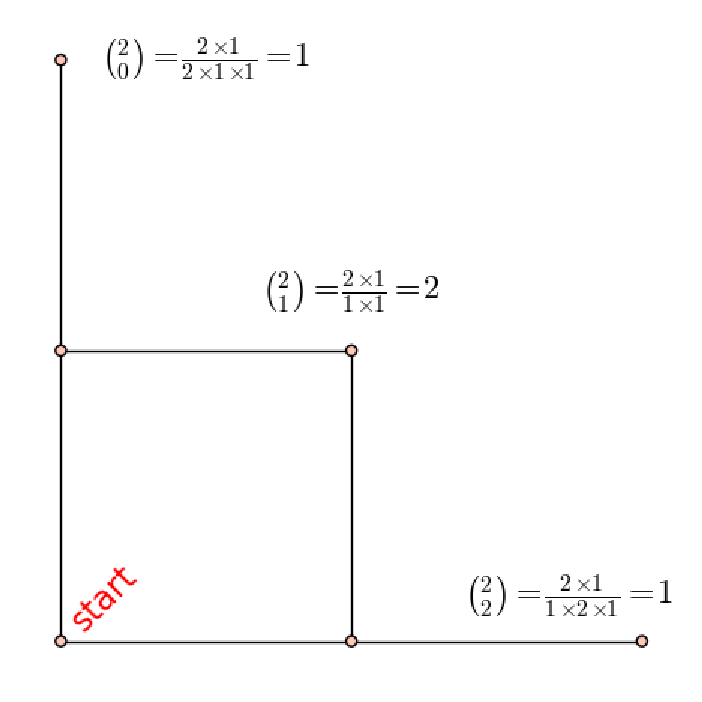
\includegraphics[width=7cm]{figures/TwoBlocksNorthEast.eps}}
\subfigure[{\scriptsize Walking three blocks north-easterly.}]{
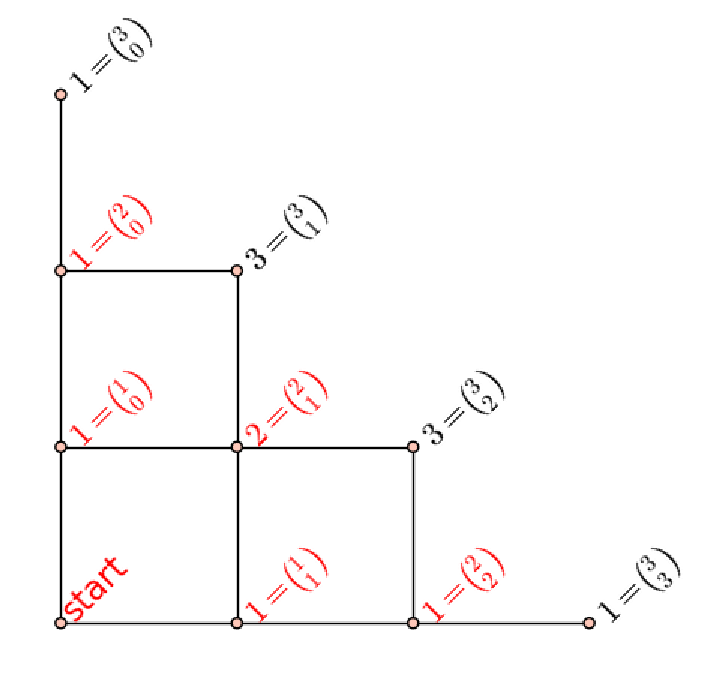
\includegraphics[width=7cm]{figures/ThreeBlocksNorthEast.eps}}
\end{figure}


\begin{Exercise}[title={Choosing Volunteers},label={xChoose3of50}]
Suppose we need three students to be the class representatives in this course.
Assume that everyone wants to be selected to keep it simple.
In how many ways can we choose these three people from the class of 50 students?
%\ExePart
%\Question
%\subQuestion Show that...
%\subQuestion In this question...
%\subsubQuestion Show that...
%\subsubQuestion Conclude...
%\subQuestion Conclude.
%\Question Show that if $b > 1$...
%\ExePart
%\Question What happens to if $b=1$?
\end{Exercise}
\begin{Answer}
We start by assuming that order does matter, that is, we have a
permutation, so that the number of ways we can select the three class
representatives is
\[^{50}P_3\;=\; \frac{50!}{(50-3)!}\;=\; \frac{50!}{47!}\]
But, because order doesn't matter,  all we have to do is to adjust our
permutation formula by a factor representing the number of  ways the objects could be in
order. Here,  three students can  be placed in order $3!$ ways, so
the required number of  ways of choosing the class representatives is:
\[ \frac{50!}{47!\, 3!}\;=\;
\frac{50\,.\, 49\,.\,48}{3\,.\,2\,.\,1}\;=\; 19,600\]
\end{Answer}

\medskip
Now, we give more formal definitions and notations that will help us make precise arguments faster when we study sampling schemes in Inference Theory.

\begin{definition}[Permutations and Factorials]
A {\bf permutation} of $n$ objects is an arrangement of $n$ distinct objects in a row.  For example, there are $2$ permutations of the two objects $\{1,2\}$:
\[
12, \qquad 21 \ ,
\]
and $6$ permutations of the three objects $\{a,b,c\}$:
\[
abc, \quad acb, \quad bac, \quad bca, \quad cab, \quad cba \ .
\]
Let the number of ways to choose $k$ objects out of $n$ and to arrange them in a row be denoted by $p_{n,k}$.  For example, we can choose two ($k=2$) objects out of three ($n=3$) objects, $\{a,b,c\}$, and arrange them in a row in six ways ($p_{3,2}$):
\[
ab, \quad ac, \quad ba, \quad bc, \quad ca, \quad cb \ .
\]
Given $n$ objects, there are $n$ ways to choose the left-most object, and once this choice has been made there are $n-1$ ways to select a different object to place next to the left-most one.  Thus, there are $n(n-1)$ possible choices for the first two positions.  Similarly, when $n>2$, there are $n-2$ choices for the third object that is distinct from the first two.  Thus, there are $n(n-1)(n-2)$ possible ways to choose three distinct objects from a set of $n$ objects and arrange them in a row.  In general,
\[
p_{n,k} = n(n-1)(n-2)\ldots (n-k+1)
\]
and the total number of permutations called `$n$ {\bf factorial}' and denoted by $n!$ is
\[
n! := p_{n,n} = n (n-1) (n-2)\ldots (n-n+1) = n (n-1) (n-2)\ldots (3) \ (2) \ (1) =: \prod_{i=1}^n i \ .
\]
\end{definition}

Some factorials to bear in mind
\[
0! := 1 \quad 1!=1, \quad 2!=2, \quad 3!=6, \quad 4!=24, \quad 5!=120 \quad 10!=3,628,800 \ .
\]
When $n$ is large we can get a good idea of $n!$ without laboriously carrying out the $n-1$ multiplications via Stirling's approximation ({\it Methodus Differentialis (1730), p.~137}) :
\[
n! \approxeq \sqrt{2 \pi n} \left( \frac{n}{e} \right)^n \ .
\]

\begin{definition}[Combinations]
The combinations of $n$ objects taken $k$ at a time are the possible choices of $k$ different elements from a collection of $n$ objects, disregarding order.  They are called the $k$-combinations of the collection.  The combinations of the three objects $\{a,b,c\}$ taken two at a time, called the $2$-combinations of $\{a,b,c\}$, are
\[
ab, \quad ac, \quad bc \ ,
\]
and the combinations of the five objects $\{1,2,3,4,5\}$ taken three at a time, called the $3$-combinations of $\{1,2,3,4,5\}$ are
\[
123, \quad 124, \quad 125, \quad 134, \quad 135, \quad 145, \quad 234, \quad 235, \quad 245, \quad 345 \ .
\]
The total number of $k$-combination of $n$ objects, called a {\bf binomial coefficient}, denoted $\binom{n}{k}$ and read ``$n$ choose $k$,'' can be obtained from $p_{n,k} = n(n-1)(n-2)\ldots(n-k+1)$ and $k! := p_{k,k}$.  Recall that $p_{n,k}$ is the number of ways to choose the first $k$ objects from the set of $n$ objects and arrange them in a row with regard to order.  Since we want to disregard order and each $k$-combination appears exactly $p_{k,k}$ or $k!$ times among the $p_{n,k}$ many permutations, we perform a division:
\[
\binom{n}{k} := \frac{p_{n,k}}{p_{k,k}} = \frac{n(n-1)(n-2)\ldots(n-k+1)}{k(k-1)(k-2)\ldots 2 \ 1} \ .
\]
\end{definition}
Binomial coefficients are often called ``Pascal's Triangle''  and attributed to Blaise Pascal's  {\it Trait\'e du Triangle Arithm\'etique} from 1653, but they have many ``fathers''.  There are earlier treatises of the binomial coefficients including Szu-y\"uan Y\"u-chien (``The Precious Mirror of the Four Elements'') by the Chinese mathematician Chu Shih-Chieh in 1303, and in an ancient Hindu classic, {\it Pi\.ngala's Chanda\d{h}\'s\=astra}, due to Hal\=ayudha (10-th century AD).



\section{Array, Sequence, Limit, \ldots}\label{S:ArraysSequencesLimitEtc}

In this section we will study a basic data structure in \Matlab called an {\bf array} of numbers.  Arrays are finite sequences and they can be processed easily in \Matlab.  The notion of infinite sequences lead to {\bf limits}, one of  the most fundamental concepts in mathematics.

For any natural number $n$, we write
$$\boxed{\langle x_{1:n} \rangle := x_1,x_{2},\ldots,x_{n-1},x_n}$$
to represent the {\bf finite sequence} of real numbers $x_1,x_2,\ldots ,x_{n-1},x_n$.
For two integers $m$ and $n$ such that $m \leq n$, we write
$$\boxed{\langle x_{m:n} \rangle := x_m,x_{m+1},\ldots,x_{n-1},x_n}$$
to represent the {\bf finite sequence} of real numbers $x_m,x_{m+1},\ldots ,x_{n-1},x_n$.  In mathematical analysis, finite sequences and their countably infinite counterparts play a fundamental role in limiting processes.  Given an integer $m$, we denote an {\bf infinite sequence} or simply a sequence as:
\[
\boxed{
\langle x_{m:\infty} \rangle := x_m, x_{m+1}, x_{m+2}, x_{m+3}, \ldots \ . }
\]
Given index set $\mathcal{I}$ which may be finite or infinite in size, a sequence can either be seen as a set of ordered pairs:
\[
\{ (i,x_i) : i \in \mathcal{I} \} \enspace ,
\]
or as a function that maps the index set to the set of real numbers:
\[
x(i)= x_i : \mathcal{I} \to \{x_{i} : i \in \mathcal{I} \} \ ,
\]
The finite sequence $\langle x_{m:n} \rangle$ has $\mathcal{I}= \{ m,m+1,m+2,m+3,\ldots,n \}$ as its index set  while an infinite sequence $\langle x_{m:\infty} \rangle$ has $\mathcal{I}= \{ m,m+1,m+2,m+3,\ldots \}$ as its index set.  A {\bf sub-sequence} $\langle x_{j:k} \rangle$ of a finite sequence $\langle x_{m:n} \rangle$ or an infinite sequence $\langle x_{m:\infty} \rangle$ is:
\[
\langle x_{j:k} \rangle = x_j,x_{j+1},\ldots,x_{k-1},x_{k} \quad \text{where, } \quad m \leq j \leq k \leq n < \infty \enspace .
\]

A rectangular arrangement of $m \cdot n$ real numbers in $m$ rows and $n$ columns is called an $m \times n$ {\bf matrix}.  The `$m \times n$' represents the {\bf size} of the matrix.  We use bold upper-case letters to denote matrices, for e.g:
$$
\X = \begin{bmatrix}
x_{1,1} & x_{1,2} & \ldots & x_{1,n-1} & x_{1,n} \\
x_{2,1} & x_{2,2} & \ldots & x_{2,n-1} & x_{2,n} \\
\vdots & \vdots & \ddots & \vdots & \vdots \\
x_{m-1,1} & x_{m-1,2} & \ldots & x_{m-1,n-1} & x_{m-1,n} \\
x_{m,1} & x_{m,2} & \ldots & x_{m,n-1} & x_{m,n}
\end{bmatrix}
$$
Matrices with only one row or only one column are called {\bf vectors}.  An $1 \times n$ matrix is called a {\bf row vector} since there is only one row and an $m \times 1$ matrix is called a {\bf column vector} since there is only one column.  We use bold-face lowercase letters to denote row and column vectors.
$$
\text{A row vector } \x = \begin{bmatrix}
x_{1} & x_{2} & \ldots & x_{n}
\end{bmatrix} = (x_1,x_2,\ldots,x_n)
$$
$$
\text{ and a column vector } \y =
\begin{bmatrix}
y_{1} \\
y_{2}  \\
\vdots \\
y_{m-1} \\
y_{m}
\end{bmatrix}
= \begin{bmatrix}
y_{1} & y_{2} & \ldots & y_{m}
\end{bmatrix}'
= (y_1,y_2,\ldots,y_m)' \ .
$$
The superscripting by $'$ is the transpose operation and simply means that the rows and columns are exchanged.  Thus the transpose of the matrix $\X$ is:
$$
\X' = \begin{bmatrix}
x_{1,1} & x_{2,1} & \ldots & x_{m-1,1} & x_{m,1} \\
x_{1,2} & x_{2,2} & \ldots & x_{m-1,2} & x_{m,2} \\
\vdots & \vdots & \ddots & \vdots & \vdots \\
x_{1,n-1} & x_{2,n-1} & \ldots & x_{m-1,n-1} & x_{m,n-1} \\
x_{1,n} & x_{2,n} & \ldots & x_{m-1,n} & x_{m,n}
\end{bmatrix}
$$
In linear algebra and calculus, it is natural to think of vectors and matrices as points (ordered $m$-tuples) and ordered collection of points in Cartesian co-ordinates.  We assume that the reader has heard of operations with matrices and vectors such as matrix multiplication, determinants, transposes, etc.  Such concepts will be introduced as they are needed in the sequel.

Finite sequences, vectors and matrices can be represented in a computer by an elementary data structure called an {\bf array}.

\begin{labwork}[Sequences as arrays]\label{LW:Seqs}
Let us learn to represent, visualise and operate finite sequences as \Matlab arrays.  Try out the commands and read the comments for clarification.
\begin{VrbM}
>> a = [17]			% Declare the sequence of one element 17 in array a
a =    17
>> % Declare the sequence of 10 numbers in array b
>> b=[-1.4508 0.6636 -1.4768 -1.2455 -0.8235 1.1254 -0.4093 0.1199 0.2043 -0.8236]
b =
   -1.4508    0.6636   -1.4768   -1.2455   -0.8235    1.1254   -0.4093    0.1199    0.2043   -0.8236
>> c = [1 2 3] 		% Declare the sequence of 3 consecutive numbers 1,2,3
c =     1     2     3
>> % linspace(x1, x2, n) generates n points linearly spaced between x1 and x2
>> r = linspace(1, 3, 3)		% Declare sequence r = c using linspace
r =     1     2     3
>> s1 = 1:10 % declare an array s1 starting at 1, ending by 10, in increments of 1
s =     1     2     3     4     5     6     7     8     9    10
>> s2 = 1:2:10  % declare an array s2 starting at 1, ending by 10, in increments of 2
s =     1     3     5     7     9
>> s2(3) % obtain the third element of the finite sequence s2
ans =     5
>> s2(2:4) % obtain the subsequence from second to fourth elements of the finite sequence s2
ans =     3     5     7
\end{VrbM}
We may visualise (as per~\hyperref[F:StemPlotDemo1]{Figure~\ref*{F:StemPlotDemo1}}) the finite sequences $\langle b_{1:n} \rangle$ stored in the array {\tt b} as the set of ordered pairs $\{(1,b_1),(2,b_2),\ldots,(10,b_{n})\}$ representing the function $b(i)=b_i:\{1,2,\ldots,n\} \to \{b_1,b_2,\ldots,b_{n} \}$ via {\bf point plot} and {\bf stem plot}  using {\tt Matlab}'s {\tt plot} and {\tt stem} commands, respectively.

\begin{figure}[hbt]
\caption{Point plot and stem plot of the finite sequence $\langle b_{1:10} \rangle$ declared as an array.\label{F:StemPlotDemo1}}
\centering   \makebox{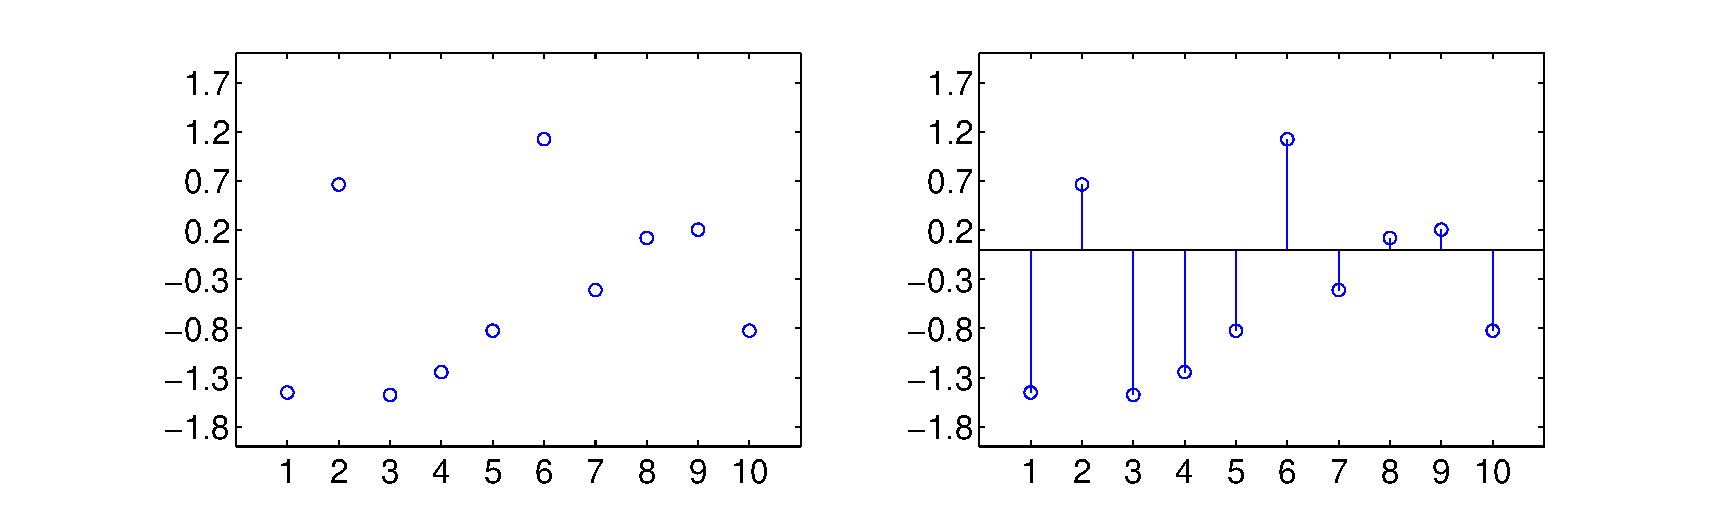
\includegraphics[width=7.0in]{figures/StemPlotDemo1}}
\end{figure}
\begin{VrbM}
>> display(b) % display the array b in memory
b =
   -1.4508    0.6636   -1.4768   -1.2455   -0.8235    1.1254   -0.4093    0.1199    0.2043   -0.8236
>> plot(b,'o') % point plot of ordered pairs (1,b(1)), (2,b(2)), ..., (10,b(10))
>> stem(b) % stem plot of ordered pairs (1,b(1)), (2,b(2)), ..., (10,b(10))
>> plot(b,'-o') % point plot of ordered pairs (1,b(1)), (2,b(2)), ..., (10,b(10)) connected by lines
\end{VrbM}
\end{labwork}

\begin{labwork}[Vectors and matrices as arrays]\label{LW:VecsMats}
Let us learn to represent, visualise and operate vectors as \Matlab arrays.  Syntactically, a vector is stored in an array exactly in the same way we stored a finite sequence.  However, mathematically, we think of a vector as an ordered $m$-tuple that can be visualised as a point in Cartesian co-ordinates.  Try out the commands and read the comments for clarification.
\begin{VrbM}
>> a = [1 2]	% an 1 X 2 row vector
>> z = [1 2 3] 	% Declare an 1 X 3 row vector z with three numbers
z =     1     2     3
>> % linspace(x1, x2, n) generates n points linearly spaced between x1 and x2
>> r = linspace(1, 3, 3)		% Declare an 1 X 3 row vector r = z using linspace
r =     1     2     3
>> c = [1; 2; 3]  	% Declare a 3 X 1 column vector c with three numbers.  Semicolons delineate columns
c =
     1
     2
     3
>> rT = r'	% The column vector (1,2,3)' by taking the transpose of r via r'
rT =
     1
     2
     3
>> y = [1 1 1] 			% y is a sequence or row vector of 3 1's
y =     1     1     1
>> ones(1,10)	% ones(m,n) is an m X n matrix of ones.  Useful when m or n is large.
ans =     1     1     1     1     1     1     1     1     1     1
\end{VrbM}
We can use two dimensional arrays to represent matrices.  Some useful built-in commands to generate standard matrices are:
\begin{VrbM}
>> Z=zeros(2,10) % the 2 X 10 matrix of zeros
Z =
     0     0     0     0     0     0     0     0     0     0
     0     0     0     0     0     0     0     0     0     0
>> O=ones(4,5) % the 4 X 5 matrix of ones
O =
     1     1     1     1     1
     1     1     1     1     1
     1     1     1     1     1
     1     1     1     1     1
>> E=eye(4) % the 4 X 4 identity matrix
E =
     1     0     0     0
     0     1     0     0
     0     0     1     0
     0     0     0     1
\end{VrbM}
We can also perform operations with arrays representing vectors, finite sequences, or matrices.
\begin{VrbM}
>> y % the array y is
y =     1     1     1
>> z % the array z is
z =     1     2     3
>> x = y + z   			% x is the sum of vectors y and z (with same size 1 X 3)
x =     2     3     4
>> y = y * 2    			% y is updated to 2 * y (each term of y is multiplied by 2)
y =     2     2     2
>> p = z .* y   			% p is the vector obtained by term-by-term product of z and y
p =     2     4     6
>> d = z ./ y    			% d is the vector obtained by term-by-term division of z and y
d =    0.5000    1.0000    1.5000
>> t=linspace(-10,10,4)		% t has 4 numbers equally-spaced between -10 and 10
t =  -10.0000   -3.3333    3.3333   10.0000
>> s = sin(t) 			% s is a vector obtained from the term-wise sin of the vector t
s =    0.5440    0.1906   -0.1906   -0.5440
>> sSq = sin(t) .^ 2	 % sSq is an array obtained from term-wise squaring ( .^ 2) of the sin(t) array
sSq =    0.2960    0.0363    0.0363    0.2960
>> cSq = cos(t) .^ 2 % cSq is an array obtained from term-wise squaring ( .^ 2) of the cos(t) array
cSq =    0.7040    0.9637    0.9637    0.7040
>> sSq + cSq % we can add the two arrays sSq and cSq to get the array of 1's
ans =     1     1     1     1
>> n = sin(t) .^2 + cos(t) .^2 	% we can directly do term-wise operation sin^2(t) + cos^2(t) of t as well
n =     1     1     1     1
>> t2 = (-10:6.666665:10)	% t2 is similar to t above but with ':' syntax of (start:increment:stop)
t2 =  -10.0000   -3.3333    3.3333   10.0000
\end{VrbM}

Similarly, operations can be performed with matrices.
\begin{VrbM}
>>  (O+O) .^ (1/2) % term-by-term square root of the matrix obtained by adding O=ones(4,5) to itself
ans =
    1.4142    1.4142    1.4142    1.4142    1.4142
    1.4142    1.4142    1.4142    1.4142    1.4142
    1.4142    1.4142    1.4142    1.4142    1.4142
    1.4142    1.4142    1.4142    1.4142    1.4142
\end{VrbM}
We can access specific rows or columns of a matrix as follows:
\begin{VrbM}
>> % declare a 3 X 3 array A of row vectors
>> A = [0.2760    0.4984    0.7513; 0.6797    0.9597    0.2551; 0.1626    0.5853    0.6991]
A =
    0.2760    0.4984    0.7513
    0.6797    0.9597    0.2551
    0.1626    0.5853    0.6991
>> A(2,:) % access the second row of A
ans =
    0.6797    0.9597    0.2551
>> B = A(2:3,:) % store the second and third rows of A in matrix B
B =
    0.6797    0.9597    0.2551
    0.1626    0.5853    0.6991
>> C = A(:,[1 3]) % store the first and third columns of A in matrix C
C =
    0.2760    0.7513
    0.6797    0.2551
    0.1626    0.6991\end{VrbM}
\end{labwork}

\begin{labwork}[Plotting a function as points of ordered pairs in two arrays]\label{LW:2Dplot}
Next we plot the function $sin(x)$ from several ordered pairs $(x_i,sin(x_i))$.  Here $x_i$'s are from the domain $[-2 \pi, 2 \pi]$.  We use the {\tt plot} function in \Matlab.  Create an M-file called {\tt MySineWave.m} and copy the following commands in it.  By entering {\tt MySineWave} in the command window you should be able to run the script and see the figure in the figure window.

\VrbMf[label=SineWave.m]{scripts/SineWave.m}

The plot was saved as an encapsulated postscript file from the File menu of the Figure window and is displayed below.
\begin{figure}[ht]
\vspace{2cm}
%FIX\centering   \makebox{\includegraphics[width=6.5in]{figures/sinewave}}
\caption{A plot of the sine wave over $[-2 \pi, 2 \pi]$.\label{F:sinfunction}}
\end{figure}
\end{labwork}

%\begin{classwork}
%Recall the trigonometric function $\sin$ with domain $\Rz$ and range $[-1,1]$.  We can explicitly refer to this function by writing:
%\[
%\sin : \Rz \to [-1,1]
%\]
%\begin{figure}[htpb]
%\caption{A depiction of the function $\sin$ and the inverse image $\sin^{[-1]}(0) =\{i \pi : i \in \Zz\}$.\label{F:sinfunction}}
%\vspace{5cm}
%\end{figure}
%\end{classwork}

%Continuity

\section{Elementary Real Analysis}



\subsection{Limits of Real Numbers -- A Review}\label{S:AnalysisRefresher}

%TODO
%Differentiability

%Riemann Integral


Let us first recall some elementary ideas from real analysis.
\begin{definition}[Convergent sequence of real numbers]\label{Dfn:ConvReals}
A sequence of real numbers  $\langle x_i \rangle_{i=1}^{\infty} := x_1,x_2,\ldots$ is said to converge to a limit $a \in \Rz$ and denoted by:
\[
\lim_{i \to \infty} x_i = a \ ,
\]
if for every natural number $m \in \Nz$, a natural number $N_m \in \Nz$ exists such that for every $j \geq N_m$, $|x_j-a| \leq \frac{1}{m}$.
\end{definition}

In words, $\lim_{i \to \infty} x_i = a$ means the following: no matter how small you make $\frac{1}{m}$ by picking as large an $m$ as you wish, I can find an $N_m$, that may depend on $m$, such that every number in the sequence beyond the $N_m$-th element is within distance $\frac{1}{m}$ of the limit $a$.

\begin{example}[Limit of a sequence of $17$s]\label{EX:limOf17s}
Let $\langle x_i \rangle_{i=1}^{\infty} = 17, 17, 17, \ldots$. Then $\lim_{i \to \infty} x_i = 17$.  This is because for every  $m \in \Nz$, we can take $N_m=1$ and satisfy the definition of the limit, i.e.:
\[
\text{for every }  j \geq N_m= 1, \  |x_j-17|=|17-17|=0\leq \frac{1}{m} \ .
\]
\end{example}

\begin{example}[Limit of $1/i$]\label{EX:limin1overi}
Let $\langle x_i \rangle_{i=1}^{\infty} = \frac{1}{1},\frac{1}{2},\frac{1}{3}, \ldots$, i.e.~$x_i = \frac{1}{i}$, then $\lim_{i \to \infty} x_i = 0$.  This is because for every  $m \in \Nz$, we can take $N_m=m$ and satisfy the definition of the limit, i.e.:
\[
\text{for every }  j \geq N_m= m, \  |x_j-0|=\left| \frac{1}{j}-0 \right|=\frac{1}{j} \leq \frac{1}{m} \ .
\]
\end{example}
However, several other sequences also approach the limit $0$.  Some such sequences that approach the limit $0$ from the right are:
\begin{flalign*}
\langle x_{1:\infty} \rangle =  \frac{1}{1},\frac{1}{4},\frac{1}{9}, \ldots \qquad \text{and} \qquad  \langle x_{1:\infty} \rangle  =  \frac{1}{1},\frac{1}{8},\frac{1}{27},\ldots \enspace ,
\end{flalign*}
and some that approach the limit $0$ from the left are:
\begin{flalign*}
\langle x_{1:\infty} \rangle =  -\frac{1}{1},-\frac{1}{2},-\frac{1}{3}, \ldots \qquad \text{and} \qquad
\langle x_{1:\infty} \rangle =  -\frac{1}{1},-\frac{1}{4},-\frac{1}{9}, \ldots \enspace ,
\end{flalign*}
and finally some that approach $0$ from either side are:
\begin{flalign*}
\langle x_{1:\infty} \rangle =  -\frac{1}{1},+\frac{1}{2},-\frac{1}{3}, \ldots \qquad \text{and} \qquad
\langle x_{1:\infty} \rangle = -\frac{1}{1},+\frac{1}{4},-\frac{1}{9} \ldots \enspace .
\end{flalign*}
When we do not particularly care about the specifics of a sequence of real numbers $\langle x_{1:\infty} \rangle$, in terms of the exact values it takes for each $i$, but we are only interested that it converges to a limit $a$ we write:
\[
x \to a
\]
and say that $x$ approaches $a$.  If we are only interested in those sequences that converge to the limit $a$ from the right or left, we write:
\[
x \to a^+ \qquad \text{or} \qquad x \to a^-
\]
and say $x$ approaches $a$ from the right or left, respectively.

\begin{definition}[Limits of Functions]\label{D:LimitofRealFunction}
We say a function $f(x):\Rz \to \Rz$ has a {\bf limit} $L \in \Rz$ as $x$ approaches $a$ and write:
\[
\lim_{x \to a} f(x)=L \ ,
\]
provided $f(x)$ is arbitrarily close to $L$ for all values of $x$ that are sufficiently close to, but not equal to, $a$.  We say that $f$ has a {\bf right limit} $L_R$ or {\bf left limit} $L_L$ as $x$ approaches $a$ from the left or right, and write:
\[
\lim_{x \to a^+} f(x)=L_R  \qquad \text{ or } \qquad \lim_{x \to a^-} f(x)=L_L \ ,
\]
provided $f(x)$ is arbitrarily close to $L_R$ or $L_L$ for all values of $x$ that are sufficiently close to, but not equal to, $a$ from the right of $a$ or the left of $a$, respectively.  When the limit is not an element of $\Rz$ or when the left and right limits are distinct, we say that the limit does not exist.
\end{definition}

\begin{example}[Limit of $1/x^2$]
Consider the function $f(x)=\frac{1}{x^2}$.  Then
\[
\lim_{x \to 1} f(x) = \lim_{x \to 1} \frac{1}{x^2} = 1
\]
exists since the limit $1 \in \Rz$, and the right and left limits are the same:
\[
\lim_{x \to 1^+} f(x) = \lim_{x \to 1^+} \frac{1}{x^2} = 1 \qquad \text{and} \qquad
\lim_{x \to 1^-} f(x) = \lim_{x \to 1^-} \frac{1}{x^2} = 1 \ .
\]
However, the following limit does not exist:
\[
\lim_{x \to 0} f(x) = \lim_{x \to 0} \frac{1}{x^2} = \infty
\]
since $\infty \notin \Rz$.
\end{example}

Let us next look at some limits of functions that exist despite the function itself being undefined at the limit point.

\begin{example}[Limit of $(1+x)^{\frac{1}{x}}$]\label{EX:LimitToE}
The limit of $f(x)=(1+x)^{\frac{1}{x}}$ as $x$ approaches $0$ exists and it is the Euler's constant $e$ :
\begin{eqnarray*}
\lim_{x \to 0} f(x)
&=& \lim_{x \to 0} (1+x)^{\frac{1}{x}}\\
&=& \lim_{x \to 0} (x+1)^{(1/x)} \quad \text{Indeterminate form of type $1^\infty$.}\\
&=& \exp\left(\lim_{x\to 0} \log((x+1)^{(1/x)})\right) \quad \text{Transformed using $\exp(\lim_{x\to 0} \log((x+1)^{(1/x)}))$} \\
&=& \exp\left(\lim_{x\to 0} (\log(x+1))/x\right) \quad \text{Indeterminate form of type $0/0$.}\\
&=& \exp\left( \lim_{x\to 0} \frac{ d\log(x+1)/ dx}{ dx/ dx} \right) \quad \text{Applying L'Hospital's rule} \\
&=&  \exp\left(\lim_{x\to 0} 1/(x+1)\right) \quad \text{limit of a quotient is the quotient of the limits}\\
&=&  \exp\left(1/(\lim_{x \to 0} (x+1))\right) \quad \text{The limit of $x+1$ as $x$ approaches $0$ is $1$}\\
&=& \exp(1)=e \approxeq 2.71828 \enspace .
\end{eqnarray*}
\[
\lim_{x \to 0} f(x) = \lim_{x \to 0} (1+x)^{\frac{1}{x}} = e \approxeq 2.71828 \ .
\]
Notice that the above limit exists despite the fact that $f(0) = (1+0)^{\frac{1}{0}}$ itself is undefined and does not exist.
\end{example}

\begin{example}[Limit of $\frac{x^3-1}{x-1}$]
For $f(x)=\frac{x^3-1}{x-1}$, this limit exists:
\[
\lim_{x \to 1} f(x) = \lim_{x \to 1} \frac{x^3-1}{x-1}
=  \lim_{x \to 1} \frac{(x-1)(x^2+x+1)}{(x-1)}
= \lim_{x \to 1} x^2+x+1 = 3 \,
\]
despite the fact that $f(1)=\frac{1^3-1}{1-1}=\frac{0}{0}$ itself is undefined and does not exist.
\end{example}

Next we look at some examples of limits at infinity.
\begin{example}[Limit of $(1-\frac{\lambda}{n})^n$]\label{EX:LimitExpofLambda}
The limit of $f(n)=\left( 1-\frac{\lambda}{n} \right)^n$ as $n$ approaches $\infty$ exists and it is $e^{-\lambda}$ :
\[
\lim_{n \to \infty} f(n) = \lim_{n \to \infty} \left( 1-\frac{\lambda}{n} \right)^n = e^{-\lambda} \ .
\]
\end{example}

\begin{example}[Limit of $(1-\frac{\lambda}{n})^{-\alpha}$]\label{EX:Limit1MinusLambdaOverNToMinusK}
The limit of $f(n)=\left( 1-\frac{\lambda}{n} \right)^{-\alpha}$, for some $\alpha>0$, as $n$ approaches $\infty$ exists and it is $1$ :
\[
\lim_{n \to \infty} f(n) = \lim_{n \to \infty} \left( 1-\frac{\lambda}{n} \right)^{-\alpha} = 1 \ .
\]
\end{example}

\begin{definition}[Continuity of a function]
We say a real-valued function $f(x):D \to \Rz$ with the domain $D \subset \Rz$ is {\bf right continuous} or {\bf left continuous} at a point $a \in D$, provided:
\[
\lim_{x \to a^+} f(x) = f(a) \qquad \text{ or } \qquad
\lim_{x \to a^-} f(x) = f(a) \ ,
\]
respectively.  We say $f$ is {\bf continuous} at $a \in D$, provided:
\[
\lim_{x \to a^+} f(x) = f(a) =
\lim_{x \to a^-} f(x) \ .
\]
Finally, $f$ is said to be continuous if $f$ is continuous at every $a \in D$.
\end{definition}
\begin{example}[Discontinuity of $f(x)=(1+x)^{\frac{1}{x}}$ at $0$]
Let us reconsider the function $f(x)=(1+x)^{\frac{1}{x}}:\Rz \to \Rz$.  Clearly, $f(x)$ is continuous at $1$, since:
\[
\lim_{x \to 1} f(x) = \lim_{x \to 1}(1+x)^{\frac{1}{x}} = 2 = f(1)=(1+1)^{\frac{1}{1}} \ ,
\]
but it is not continuous at $0$, since:
\[
\lim_{x \to 0} f(x) = \lim_{x \to 0} (1+x)^{\frac{1}{x}} = e \approxeq 2.71828 \neq f(0) = (1+0)^{\frac{1}{0}} \ .
\]
Thus, $f(x)$ is not a continuous function over $\Rz$.
\end{example}

%Here is a summary of the notations we have learned here.
%\begin{table}[t]
%\centering
%\begin{tabular}{cc}
%$\Omega$&\\
%$\to$&\\
%$f^{[-1]}$&\\
%$lim _{i\to \infty}x_i=a$&\\
%${x_i}^\infty_{i=1}$&\\
%$a^+$ and $a^-$&\\
%$\approxeq$ & \\
%\end{tabular}
%%\caption{}
%%\label{tab:}
%\end{table}

%\begin{table}[htb]
%\centering
%{\normalsize
%\begin{tabular}{| l | l |}
%\hline
%Symbol & Meaning\\ \hline
%$\Nz$& The set of natural numbers $\{1,2,3,\ldots\}$\\
%$\Zz$&The set of integers $\{\ldots,-3,-2,-1,0,1,2,3,\ldots\}$\\
%$\Dz_+$& The set of non-negative integers $\{0,1,2,3,\ldots\}$\\
%$\Rz$& The set of real numbers\\ \hline
%\end{tabular}
%}
%\caption{Analysis Symbol Table \label{T:SymbTableAnalysis}}
%\end{table}

\section{Elementary Number Theory}\label{S:ElemNumTh}
We introduce basic notions that we need from elementary number theory here.  These notions include integer functions and modular arithmetic as they will be needed later on.

For any real number $x$:
\begin{flalign*}
\lfloor x \rfloor &:= \max\{y: y \in \Zz \text{ and } y \leq x\}, \text{i.e., the greatest integer less than or equal to $x$ (the {\bf floor} of $x$),}\\
\lceil x \rceil &:= \min\{y: y \in \Zz \text{ and } y \geq x\}, \text{i.e., the least integer greater than or equal to $x$ (the {\bf ceiling} of $x$).}
\end{flalign*}

\begin{example}[Floors and ceilings]
\[
\lfloor 1 \rfloor = 1, \quad \lceil 1 \rceil = 1, \quad \lfloor 17.8 \rfloor = 17, \quad   \lfloor -17.8 \rfloor = -18, \quad \lceil \sqrt{2} \rceil = 2, \quad \lfloor \pi \rfloor = 3, \quad \lceil \frac{1}{10^{100}} \rceil = 1.
\]
\end{example}

\begin{labwork}[Floors and ceilings in \Matlab]\label{LW:FloorCeil}  We can use \Matlab functions {\tt floor} and {\tt ceil} to compute $\lfloor x \rfloor$ and $\lceil x \rceil$, respectively.  Also, the argument  $x$ to these functions can be an array.
\begin{VrbM}
>> sqrt(2) % the square root of 2 is
ans =    1.4142
>> ceil(sqrt(2)) % ceiling of square root of 2
ans =     2
>> floor(-17.8) % floor of -17.8
ans =   -18
>> ceil([1 sqrt(2) pi -17.8 1/(10^100)]) %the ceiling of each element of an array
ans =     1     2     4   -17     1
>> floor([1 sqrt(2) pi -17.8 1/(10^100)]) % the floor of each element of an array
ans =     1     1     3   -18     0
\end{VrbM}
\end{labwork}

\begin{classwork}[Relations between floors and ceilings]
Convince yourself of the following formulae.  Use examples, plots and/or formal arguments.
\begin{flalign*}
\lceil x \rceil &= \lfloor x \rfloor \iff x \in \Zz \\
\lceil x \rceil &= \lfloor x \rfloor + 1 \iff x \notin \Zz \\
\lfloor -x \rfloor &= - \lceil x \rceil \\
x-1 < \lfloor x \rfloor \leq x & \leq \lceil x \rceil < x+1
\end{flalign*}
\end{classwork}

Let us define modular arithmetic next.  Suppose $x$ and $y$ are any real numbers, i.e.~$x,y \in \Rz$, we define the binary operation called ``$x \mod y$'' as:
\[
x \mod y :=
\begin{cases}
x - y \lfloor x/y \rfloor & \text{if $y \neq 0$} \\
x  & \text{if $y = 0$}
\end{cases}
\]
%} % end of remove
